% AutoMaze AI - Livrable 1 : dossier Go/noGo
% Structure : introduction générale, six chapitres, conclusion, bibliographie et annexes
% (voir livrables/architecture_gonogo_attendue.txt).
% Compilation depuis ce dossier : pdflatex main.tex (deux fois, pour le sommaire et les renvois)
\documentclass[11pt,a4paper]{report}

\usepackage[T1]{fontenc}
\usepackage[utf8]{inputenc}
\usepackage{lmodern}
\usepackage[french]{babel}
\usepackage[a4paper,margin=2.5cm]{geometry}
\usepackage{amsmath,amssymb}
\usepackage{array,booktabs,tabularx}
\usepackage{enumitem}
\usepackage{graphicx}
\usepackage{float}
\usepackage[table]{xcolor}
\usepackage{caption}
\usepackage{subcaption}
\usepackage{tikz}
\usetikzlibrary{arrows.meta,positioning,calc,shapes.geometric,fit,babel}
\usepackage{titlesec}
\usepackage{hyperref}

\hypersetup{
  colorlinks=true,
  linkcolor=black,
  urlcolor=blue!60!black,
  pdftitle={AutoMaze AI - Livrable 1 : dossier Go/noGo},
  pdfauthor={Equipe AutoMaze AI}
}

% Chapitres plus compacts que le style par défaut de la classe report
\titleformat{\chapter}[display]{\normalfont\huge\bfseries}{\large\chaptertitlename~\thechapter}{0.4em}{}
\titlespacing*{\chapter}{0pt}{-1.5em}{1.5em}

\graphicspath{{figures/img/}}

\setlength{\parindent}{0pt}
\setlength{\parskip}{0.6em}
\renewcommand{\arraystretch}{1.25}
\setlist{itemsep=0.2em,topsep=0.2em}
\captionsetup{font=small,labelfont=bf}

% Colonne de tableau qui s'adapte à la largeur, alignée à gauche
\newcolumntype{Y}{>{\raggedright\arraybackslash}X}

% Tout ce qui reste à compléter ressort en orange : à chercher avant la remise
\newcommand{\acompleter}[1]{\textcolor{orange!85!black}{\textbf{[#1]}}}

% Couleurs des figures
\definecolor{accent}{HTML}{1F6FB2}
\definecolor{integration}{HTML}{2E8B57}

\begin{document}

\begin{titlepage}
  \centering
  {\large HESTIM --- Engineering \& Business School\par}
  \vspace{0.3cm}
  {\large Projet PACTE --- 4\textsuperscript{e} année\par}
  \vspace{0.3cm}
  {Année universitaire 2026--2027\par}

  \vspace{3cm}
  {\Huge\bfseries AutoMaze AI\par}
  \vspace{0.6cm}
  {\Large Classification d'objets routiers par Machine Learning\\pour les véhicules autonomes\par}

  \vspace{1.5cm}
  {\LARGE\bfseries Livrable 1 : dossier Go/noGo\par}

  \vfill
  \begin{tabular}{ll}
    \textbf{Équipe :} & Rodrigue Nzuzi \\
                      & \acompleter{Membre 2} \\
                      & \acompleter{Membre 3} \\[0.4em]
    \textbf{Encadrant :} & \acompleter{Nom de l'encadrant} \\[0.4em]
    \textbf{Date :} & 4 novembre 2026 \\
  \end{tabular}
\end{titlepage}


\tableofcontents

\section{Introduction}
\label{sec:introduction}

Pour conduire seul, un véhicule doit d'abord comprendre ce qu'il a devant lui. Face à un piéton, il doit s'arrêter ; face à un camion immobile, il vaut mieux le contourner. Reconnaître ce qui se trouve sur la route est donc une étape essentielle de sa perception, et c'est à cette étape que s'intéresse notre projet PACTE de 4\textsuperscript{e} année à HESTIM.

Le sujet nous demande de choisir un jeu de données, de comparer plusieurs modèles de Machine Learning et de comprendre quelles classes leur posent le plus de difficultés. Nous devrons ensuite tester le modèle final sur des images qu'il n'a jamais vues. Ce dossier explique comment nous comptons nous y prendre et prépare la décision de Go/noGo, qui représente 15~\% de la note finale.

\chapter{Présentation du projet et cahier des charges}
\label{chap:projet}

\section{Introduction}

Avant toute réalisation technique, il est essentiel de définir le cadre général du projet, ses objectifs, les besoins à satisfaire et la méthode à suivre. Le cahier des charges constitue la base du travail en précisant les aspects fonctionnels, organisationnels et techniques qui orienteront la suite du projet. Dans le cadre du \textbf{projet PACTE}, il permet d'identifier les attentes liées au sujet, de les traduire en exigences concrètes et de déterminer les contraintes à respecter. Ce chapitre présente donc le projet, sa problématique, ses objectifs, son périmètre, les besoins fonctionnels et non fonctionnels ainsi que la méthodologie et le planning prévisionnel.

\section{Présentation et contexte}

Ce projet a pour objectif de concevoir un système capable de reconnaître, à partir de l'image d'un objet, six usagers de la route : la \textbf{personne}, le \textbf{vélo}, la \textbf{voiture}, la \textbf{moto}, le \textbf{bus} et le \textbf{camion}. Pour chaque image, le modèle renvoie une classe ainsi qu'un \textbf{score de confiance}. Une fois entraîné, il est testé sur des images qu'il n'a jamais vues, puis utilisé par un véhicule virtuel qui circule dans les vraies rues de Casablanca.

Le projet place l'équipe dans la position d'une cellule de développement chargée de mettre en œuvre la brique de perception d'un véhicule autonome. Notre équipe est composée de trois étudiants, chacun étant responsable d'un rôle précis.

\begin{table}[H]
\centering
\caption{Répartition des rôles au sein de l'équipe}
\label{tab:roles}
\begin{tabularx}{\textwidth}{>{\raggedright\arraybackslash}p{3.8cm}>{\raggedright\arraybackslash}p{3.6cm}Y}
  \toprule
  \entete \textbf{Rôle} & \textbf{Responsable} & \textbf{Missions} \\
  \midrule
  Données & \acompleter{Nom} & Exploration, prétraitement, recadrages et découpage des données \\
  Modèles & \acompleter{Nom} & Extraction des caractéristiques, entraînement des classifieurs et suivi des essais \\
  Évaluation et intégration & \acompleter{Nom} & Évaluation finale, analyse des erreurs, export du modèle et lien avec le simulateur \\
  \bottomrule
\end{tabularx}
\end{table}

\section{Problématique}

Dans la plupart des systèmes de conduite autonome, la reconnaissance des usagers de la route repose sur des modèles très volumineux, entraînés sur des millions d'images et sur des machines puissantes. Dans un cadre académique, avec un \textbf{jeu de données de taille limitée}, \textbf{sans poids préentraînés} et \textbf{sans GPU dédié}, la question de la fiabilité d'un tel modèle se pose naturellement.

Le projet AutoMaze AI vise à répondre à la question suivante :

\begin{quote}
\itshape Un modèle entraîné de zéro sur un jeu de données de taille limitée peut-il reconnaître les usagers de la route de manière suffisamment fiable pour guider les décisions d'un véhicule autonome virtuel ?
\end{quote}

De cette question découlent trois interrogations complémentaires. Il s'agit d'abord de déterminer quel classifieur, parmi SVM, Random Forest et k-NN, obtient les meilleurs résultats sur les mêmes caractéristiques. Il faut ensuite identifier les classes les plus difficiles à reconnaître et comprendre pourquoi. Enfin, il est important de mesurer les conséquences d'une erreur du modèle sur le comportement du véhicule, notamment lorsqu'un piéton n'est pas reconnu.

\section{Objectifs du projet}

\subsection{Objectif général}

L'objectif principal du projet est de \textbf{développer et d'évaluer un classifieur d'objets routiers entraîné de zéro}, puis de montrer comment ses prédictions peuvent guider un \textbf{véhicule autonome virtuel} jusqu'à sa destination.

\subsection{Objectifs spécifiques}

Pour atteindre cet objectif général, plusieurs objectifs spécifiques ont été définis :

\begin{table}[H]
\centering
\caption{Objectifs spécifiques et mesures de réussite}
\begin{tabularx}{\textwidth}{l>{\raggedright\arraybackslash}p{5.8cm}Y}
  \toprule
  \entete \textbf{N°} & \textbf{Objectif spécifique} & \textbf{Mesure de réussite} \\
  \midrule
  OS1 & Décrire le jeu de données retenu & Provenance, volume, répartition par classe, résolution et qualité documentées \\
  OS2 & Préparer les images & Nettoyage, recadrage, normalisation et découpage sans fuite de données \\
  OS3 & Comparer SVM, Random Forest et k-NN & Accuracy, précision, rappel, F1 et matrice de confusion, calculés sur les mêmes données \\
  OS4 & Analyser les classes difficiles & Paires de classes confondues et images mal classées expliquées \\
  OS5 & Prédire la classe de nouvelles images & Affichage du type \og Image \textrightarrow{} Voiture (92~\%) \fg{} \\
  OS6 & Intégrer le modèle au véhicule virtuel & Chaque prédiction déclenche une décision, et les erreurs graves sont comptées \\
  \bottomrule
\end{tabularx}
\end{table}

Pour juger nos modèles, nous retenons principalement le \textbf{F1 macro}, qui accorde le même poids à chaque classe. Aucune valeur cible n'est fixée à l'avance : la référence sera le meilleur modèle classique, comparé à des scores planchers (section~\ref{sec:metriques}).

\section{Périmètre fonctionnel}
\label{sec:perimetre}

Afin d'éviter que le projet ne devienne trop vaste, nous distinguons les \textbf{fonctionnalités principales}, qui relèvent du Machine Learning et constituent le cœur scientifique du projet, des \textbf{fonctionnalités d'intégration}, qui servent à la démonstration finale.

\begin{table}[H]
\centering
\caption{Délimitation du périmètre par module}
\begin{tabularx}{\textwidth}{>{\raggedright\arraybackslash}p{3.4cm}Y>{\raggedright\arraybackslash}p{2.4cm}}
  \toprule
  \entete \textbf{Module} & \textbf{Responsabilité} & \textbf{Importance} \\
  \midrule
  Dataset & Fournir les images des objets routiers & Essentielle \\
  Prétraitement & Préparer les images pour l'apprentissage & Essentielle \\
  Classification ML & Identifier la classe d'un objet & Essentielle \\
  Évaluation & Comparer les classifieurs & Essentielle \\
  \midrule
  Simulateur & Fournir un environnement de démonstration & Intégration \\
  Localisation & Fournir les coordonnées des objets & Intégration \\
  Planification & Calculer le chemin le plus court & Intégration \\
  Décision & Choisir le comportement face aux obstacles & Intégration \\
  Contrôle & Commander le véhicule virtuel & Intégration \\
  \bottomrule
\end{tabularx}
\end{table}

Les fonctionnalités d'intégration sont nécessaires à la démonstration, mais nous veillerons à ce qu'elles ne prennent pas le dessus sur les expérimentations de Machine Learning demandées par le sujet.

\textbf{La détection d'objets reste hors périmètre.} Notre modèle ne recherche pas la position des objets dans une image complète, ce qui relèverait d'un détecteur comme YOLO ou R-CNN (figure~\ref{fig:detection}), interdit par les règles du cours. Il reçoit l'image d'un objet déjà isolé et en détermine la nature. Dans le simulateur, c'est la position connue de chaque objet qui remplace l'étape de détection. La vidéo et la physique réaliste du véhicule sont également exclues du périmètre.

\begin{figure}[H]
  \centering
  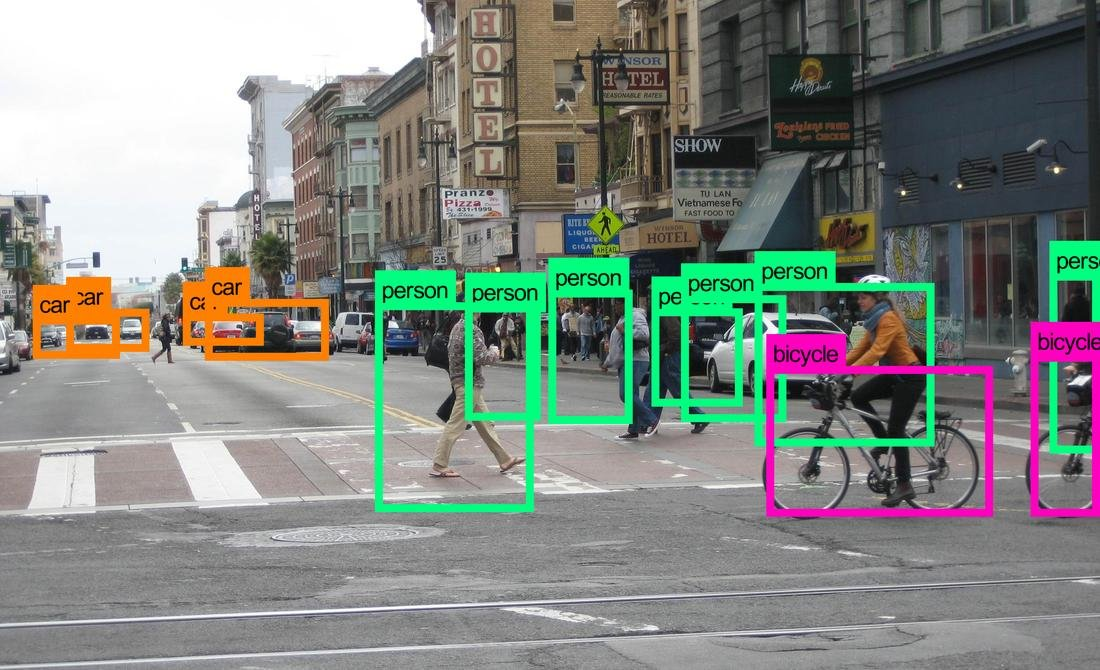
\includegraphics[width=0.68\textwidth]{dectection_dobjet_en_utilisant_regions_avec_cnn.jpg}
  \caption{Détection d'objets par réseau à régions (R-CNN), hors du périmètre de notre projet}
  \label{fig:detection}
\end{figure}

\section{Besoins fonctionnels}
\label{sec:besoins-fonctionnels}

Les besoins fonctionnels regroupent l'ensemble des fonctionnalités que le système doit offrir. Les exigences EF01 à EF06 reprennent les attentes du sujet, tandis que les exigences EF07 à EF14 concernent l'intégration dans le véhicule virtuel. Pour chacune d'elles, nous avons défini un critère d'acceptation qui permettra de vérifier qu'elle est remplie.

\begin{table}[H]
\centering
\small
\caption{Exigences fonctionnelles consolidées}
\begin{tabularx}{\textwidth}{l>{\raggedright\arraybackslash}p{5.4cm}Y}
  \toprule
  \entete \textbf{ID} & \textbf{Exigence} & \textbf{Critère d'acceptation} \\
  \midrule
  EF01 & Charger et explorer le dataset routier & Effectifs par classe, tailles et exemples présentés (notebook 01) \\
  EF02 & Prétraiter les images & Images filtrées, recadrées, redimensionnées et normalisées, découpage sans photo partagée (notebook 02) \\
  EF03 & Extraire les caractéristiques visuelles & Descripteurs HOG calculés pour toutes les images (notebook 03) \\
  EF04 & Entraîner plusieurs modèles de classification & SVM, Random Forest et k-NN entraînés sur les mêmes caractéristiques \\
  EF05 & Évaluer et comparer les modèles & Tableau commun : accuracy, précision, rappel, F1 et matrices de confusion \\
  EF06 & Prédire la classe d'un nouvel objet & Une image inconnue donne une classe et un score affichés \\
  EF07 & Récupérer les coordonnées des objets dans le simulateur & Chaque obstacle possède un tronçon de rue et une position sur ce tronçon \\
  EF08 & Associer les prédictions aux objets virtuels & Chaque prédiction est rattachée à l'obstacle dont provient l'image \\
  EF09 & Représenter les obstacles dans l'environnement & Tronçons bloqués ou pénalisés selon la décision \\
  EF10 & Calculer le chemin vers la destination avec Dijkstra & Plus court chemin trouvé sur la carte et vérifié par des tests \\
  EF11 & Adapter le trajet en présence d'un obstacle & Nouveau calcul après chaque obstacle bloquant \\
  EF12 & Décider de ralentir, s'arrêter ou contourner & Une action par classe prédite, et un arrêt prudent si le score est trop faible \\
  EF13 & Commander le véhicule virtuel & Le véhicule avance, ralentit, s'arrête, fait demi-tour ou change de rue \\
  EF14 & Afficher les prédictions et les décisions du véhicule & Image, classe, score et action visibles à l'écran \\
  \bottomrule
\end{tabularx}
\end{table}

\section{Besoins non fonctionnels}

Les besoins non fonctionnels définissent les critères de qualité et les contraintes que le système doit respecter. Ils ne concernent pas directement les fonctionnalités visibles, mais influencent fortement la fiabilité des résultats et la crédibilité du projet.

\begin{itemize}
  \item \textbf{Entraînement de zéro}\\
  Aucun YOLO, aucun détecteur et aucun poids préentraîné ne doivent être utilisés dans notre modèle.
  \item \textbf{Fiabilité de l'évaluation}\\
  Le découpage doit se faire par photo d'origine, et le jeu de test ne doit être utilisé qu'une seule fois, lors de l'évaluation finale.
  \item \textbf{Reproductibilité}\\
  Les graines aléatoires doivent être fixées, les essais notés, et les notebooks exécutables de bout en bout.
  \item \textbf{Cohérence du prétraitement}\\
  La taille des images, l'ordre des couleurs et la normalisation doivent être identiques dans les notebooks et dans le simulateur.
  \item \textbf{Séparation entre vérité terrain et perception}\\
  Les décisions du véhicule ne doivent jamais utiliser la vraie classe connue du simulateur, mais uniquement la classe prédite par le modèle.
  \item \textbf{Honnêteté des résultats}\\
  Aucune métrique ne doit être inventée. Sans modèle chargé, l'interface doit afficher \og SIMULATION --- modèle réel non chargé \fg{}.
  \item \textbf{Respect des licences}\\
  Les sources des données (COCO), de la carte (OpenStreetMap, licence ODbL) et des illustrations doivent être citées.
  \item \textbf{Temps de réponse}\\
  Une prédiction doit prendre quelques millisecondes sur un processeur ordinaire, afin de garantir une démonstration fluide.
\end{itemize}

\section{Contraintes techniques et académiques}

Le projet doit respecter plusieurs contraintes, liées à la fois au cadre du cours et aux moyens dont dispose l'équipe :

\begin{itemize}
  \item \textbf{Règles du cours}\\
  L'utilisation de YOLO, de détecteurs et de poids préentraînés est interdite pour notre modèle. Les classifieurs à comparer sont ceux du sujet : SVM, Random Forest et k-NN.
  \item \textbf{Calendrier}\\
  Le projet s'organise autour de trois échéances fixes : la séance 1 le 4 novembre, la séance 2 le 25 novembre et la soutenance le 16 décembre 2026.
  \item \textbf{Matériel}\\
  Aucun membre de l'équipe ne dispose d'un GPU. Les traitements doivent donc pouvoir s'exécuter sur un processeur ordinaire, avec le GPU gratuit de Google Colab en appui.
  \item \textbf{Budget}\\
  Le projet ne nécessite aucun budget, car l'ensemble des outils et des données retenus sont gratuits.
  \item \textbf{Licences}\\
  Les images de COCO conservent leur licence Flickr et ne sont donc pas redistribuées dans le dépôt Git.
\end{itemize}

\begin{table}[H]
\centering
\small
\caption{Ressources nécessaires au projet}
\begin{tabularx}{\textwidth}{>{\raggedright\arraybackslash}p{2.6cm}Y>{\raggedright\arraybackslash}p{4.4cm}}
  \toprule
  \entete \textbf{Ressource} & \textbf{Détail} & \textbf{Solution} \\
  \midrule
  Données & Images des 6 classes, étiquettes fiables, licence compatible & COCO 2017, à valider par l'encadrante \\
  Calcul & Entraînement des modèles & Processeur local, Google Colab en appui \\
  Stockage & Données, poids et figures partagés & Dossier Google Drive partagé \\
  Poste local & Fenêtre du simulateur, que Colab ne peut pas ouvrir & Disponible \\
  Encadrement & Validation du dataset et du périmètre & Section~\ref{sec:criteres-go} \\
  \bottomrule
\end{tabularx}
\end{table}

\section{Méthodologie et planning prévisionnel}

Pour la conduite de ce projet, nous avons retenu une démarche en \textbf{deux phases}, illustrée par la figure~\ref{fig:flux}. La première phase consiste à développer et à entraîner le modèle dans des notebooks versionnés sur GitHub. La seconde consiste à charger le modèle exporté dans le simulateur, sans jamais l'y réentraîner.

\begin{figure}[H]
  \centering
  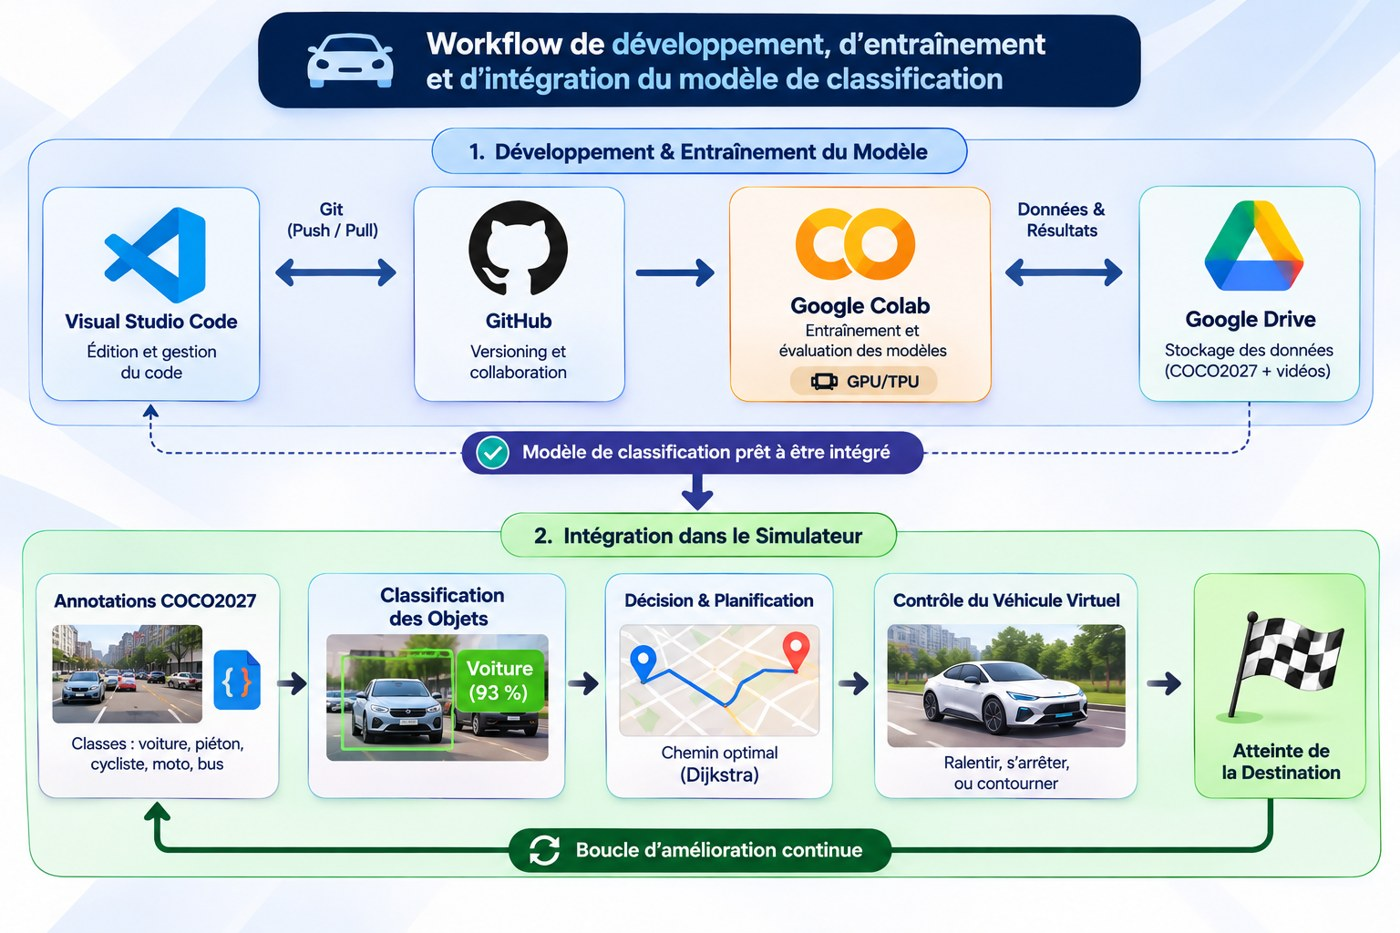
\includegraphics[width=0.9\textwidth]{flux_de_developpement_et_integration_autonome.jpg}
  \caption{Flux de développement, d'entraînement et d'intégration du modèle (lire COCO 2017, classes complétées par le camion)}
  \label{fig:flux}
\end{figure}

Cette démarche s'organise en quatre grandes étapes :

\begin{enumerate}
  \item \textbf{Données (notebooks 01 et 02)} : acquisition, exploration, nettoyage, recadrage et découpage des images.
  \item \textbf{Modèles (notebook 03)} : extraction des descripteurs HOG, puis entraînement et réglage de SVM, Random Forest et k-NN sur le jeu de validation.
  \item \textbf{Évaluation (notebook 05)} : mesure unique sur le jeu de test, analyse des erreurs et prédiction sur de nouvelles images.
  \item \textbf{Intégration} : export du modèle, branchement dans le simulateur et comparaison sur plusieurs épisodes de conduite.
\end{enumerate}

Sur le plan de l'organisation, une seule personne modifie un notebook à la fois, et chaque notebook est relu par un autre membre avant chaque séance. Les décisions importantes sont consignées dans un journal de bord. Le planning détaillé est présenté à la section~\ref{sec:planning}.

\section{Conclusion}

Ce premier chapitre a permis de définir le \textbf{cadre général du projet AutoMaze AI} en précisant son contexte, sa problématique, ses objectifs et son périmètre. L'élaboration du cahier des charges a constitué une étape essentielle pour traduire les attentes du sujet en exigences vérifiables, tout en distinguant clairement le travail de Machine Learning, qui reste au cœur du projet, des fonctionnalités d'intégration. Cette analyse préliminaire servira de base au chapitre suivant, consacré à l'analyse fonctionnelle et à la conception du système.

\chapter{Analyse fonctionnelle et conception du système}
\label{chap:analyse}

\section{Introduction}

Après avoir défini les objectifs, le périmètre et les contraintes du projet dans le cahier des charges, cette deuxième étape vise à analyser le \textbf{fonctionnement attendu du système} afin de poser les bases de sa conception. L'analyse fonctionnelle assure la cohérence entre les attentes du sujet et la structure technique de la solution. Dans un premier temps, nous identifierons les acteurs et les cas d'utilisation, puis nous décrirons les scénarios de démonstration. Nous formaliserons ensuite le comportement du système à travers les diagrammes \textbf{UML} de cas d'utilisation, d'activité, de séquence et de composants.

\section{Identification des acteurs}

L'identification des acteurs constitue une étape essentielle de l'analyse fonctionnelle. Elle permet de déterminer les différentes parties qui interagissent avec le système, chacune ayant un rôle et des responsabilités spécifiques.

\textbf{1. Équipe projet}\\
\textbf{Rôle :} l'équipe conçoit et entraîne le modèle de classification.\\
\textbf{Responsabilités :}
\begin{itemize}
  \item Préparer les données et réaliser leur découpage.
  \item Entraîner et comparer les classifieurs.
  \item Évaluer le modèle final et analyser ses erreurs.
\end{itemize}

\textbf{2. Utilisateur de la démonstration}\\
\textbf{Rôle :} l'utilisateur interagit avec le système pour observer son fonctionnement.\\
\textbf{Responsabilités :}
\begin{itemize}
  \item Classer une nouvelle image.
  \item Lancer un épisode de conduite dans le simulateur.
\end{itemize}

\textbf{3. Encadrante et jury}\\
\textbf{Rôle :} l'encadrante valide les choix du projet et suit son avancement, tandis que le jury évalue les résultats.\\
\textbf{Responsabilités :}
\begin{itemize}
  \item Valider le jeu de données et le périmètre du projet.
  \item Consulter les résultats, le rapport et la démonstration.
\end{itemize}

À ces acteurs humains s'ajoutent deux acteurs système : le \textbf{simulateur}, qui fournit l'environnement, les positions des objets et leurs images, et le \textbf{modèle ML}, qui renvoie la classe et le score d'une image.

\begin{table}[H]
\centering
\caption{Résumé des acteurs et de leurs rôles}
\begin{tabularx}{\textwidth}{>{\raggedright\arraybackslash}p{3.6cm}>{\raggedright\arraybackslash}p{2.2cm}Y}
  \toprule
  \entete \textbf{Acteur} & \textbf{Type} & \textbf{Rôle principal} \\
  \midrule
  Équipe projet & Humain & Préparation des données, entraînement et évaluation des modèles \\
  Utilisateur de la démo & Humain & Classification d'images et lancement d'épisodes de conduite \\
  Encadrante & Humain & Validation des choix et suivi de l'avancement \\
  Jury & Humain & Évaluation des résultats, du rapport et de la démonstration \\
  Simulateur & Système & Environnement, positions et images des objets \\
  Modèle ML & Système & Classe et score de chaque image \\
  \bottomrule
\end{tabularx}
\end{table}

\section{Description des cas d'utilisation}

\begin{table}[H]
\centering
\small
\caption{Description des cas d'utilisation}
\begin{tabularx}{\textwidth}{l>{\raggedright\arraybackslash}p{3.6cm}>{\raggedright\arraybackslash}p{2.4cm}Y}
  \toprule
  \entete \textbf{ID} & \textbf{Cas d'utilisation} & \textbf{Acteur} & \textbf{Résultat attendu} \\
  \midrule
  UC1 & Préparer les données & Équipe & Recadrages filtrés, normalisés et découpés en entraînement, validation et test \\
  UC2 & Entraîner et comparer les classifieurs & Équipe & Tableau comparatif de SVM, Random Forest et k-NN sur la validation \\
  UC3 & Évaluer le modèle final & Équipe, encadrante & Scores sur le test, matrice de confusion et analyse des erreurs \\
  UC4 & Classer une nouvelle image & Utilisateur & \og photo.jpg \textrightarrow{} Voiture (92~\%) \fg{} \\
  UC5 & Lancer une démonstration de conduite & Utilisateur, jury & Le véhicule rejoint sa destination en réagissant aux obstacles \\
  UC6 & Comparer les classifieurs dans le simulateur & Équipe & Collisions, fautes graves et décisions inadaptées sur plusieurs épisodes \\
  UC7 & Consulter les résultats et le rapport & Encadrante, jury & Notebooks commentés, figures et rapport \\
  \bottomrule
\end{tabularx}
\end{table}

\section{Scénarios de fonctionnement}
\label{sec:scenarios}

Ces scénarios serviront à la fois à concevoir les tests et à montrer ce que le système final devra accomplir. Les illustrations de la figure~\ref{fig:scenarios} proviennent d'autres simulateurs et servent uniquement d'inspiration. Une capture de notre propre simulateur est présentée à la section~\ref{sec:environnement}.

\begin{figure}[H]
  \centering
  \begin{subfigure}[t]{0.48\textwidth}
    \centering
    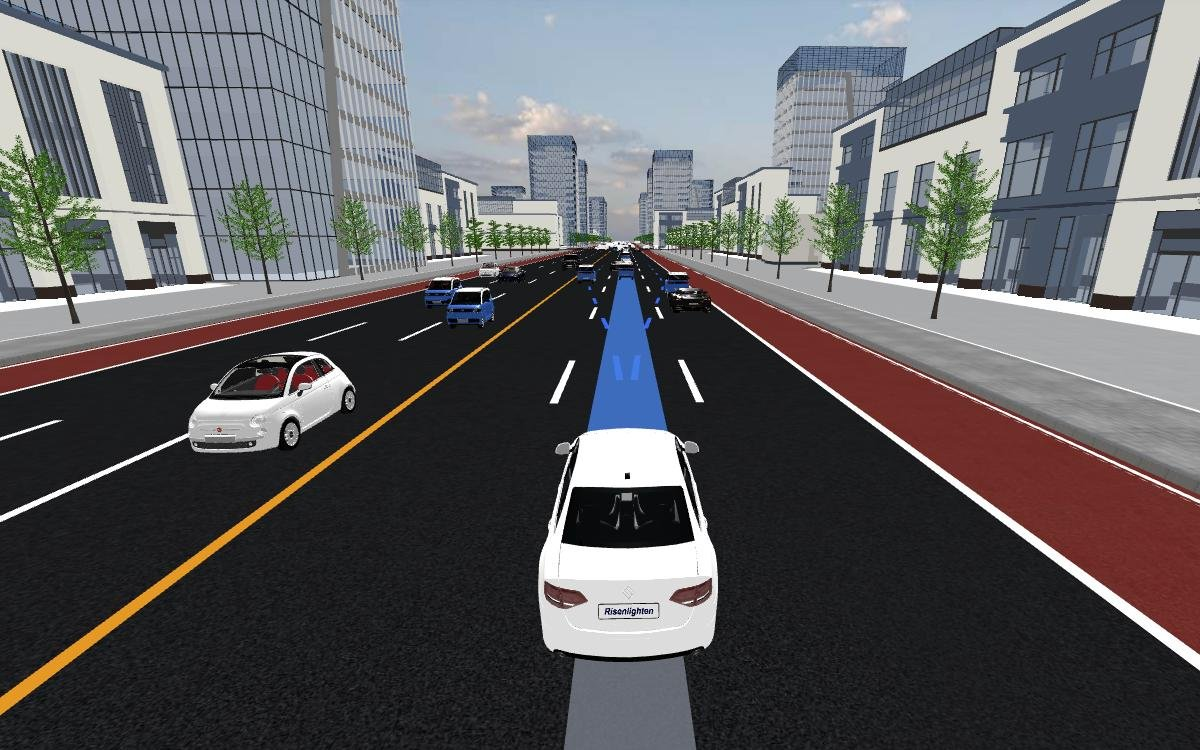
\includegraphics[width=\textwidth,height=4.2cm,keepaspectratio]{scenario1route_libre.jpg}
    \caption{Scénario 1 : route libre}
  \end{subfigure}\hfill
  \begin{subfigure}[t]{0.48\textwidth}
    \centering
    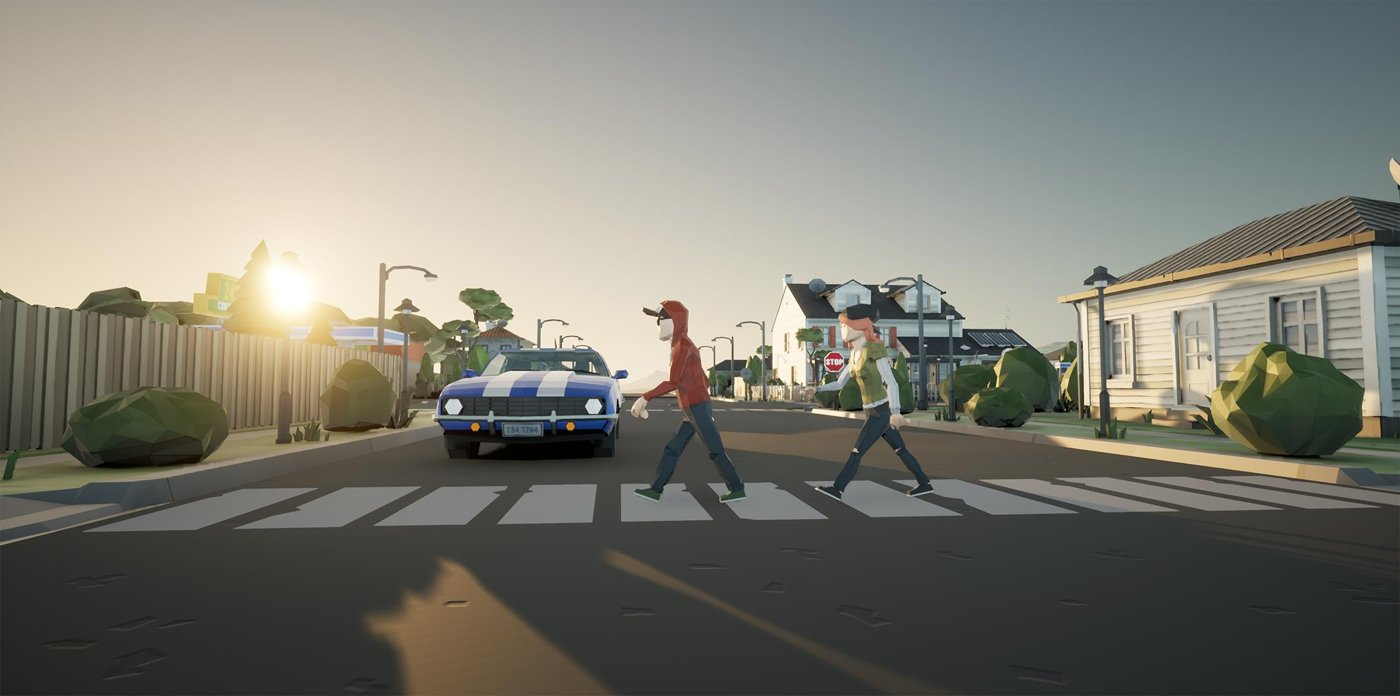
\includegraphics[width=\textwidth,height=4.2cm,keepaspectratio]{scenario2_presence_pieton.jpg}
    \caption{Scénario 2 : présence d'un piéton}
  \end{subfigure}

  \vspace{0.6em}
  \begin{subfigure}[t]{0.48\textwidth}
    \centering
    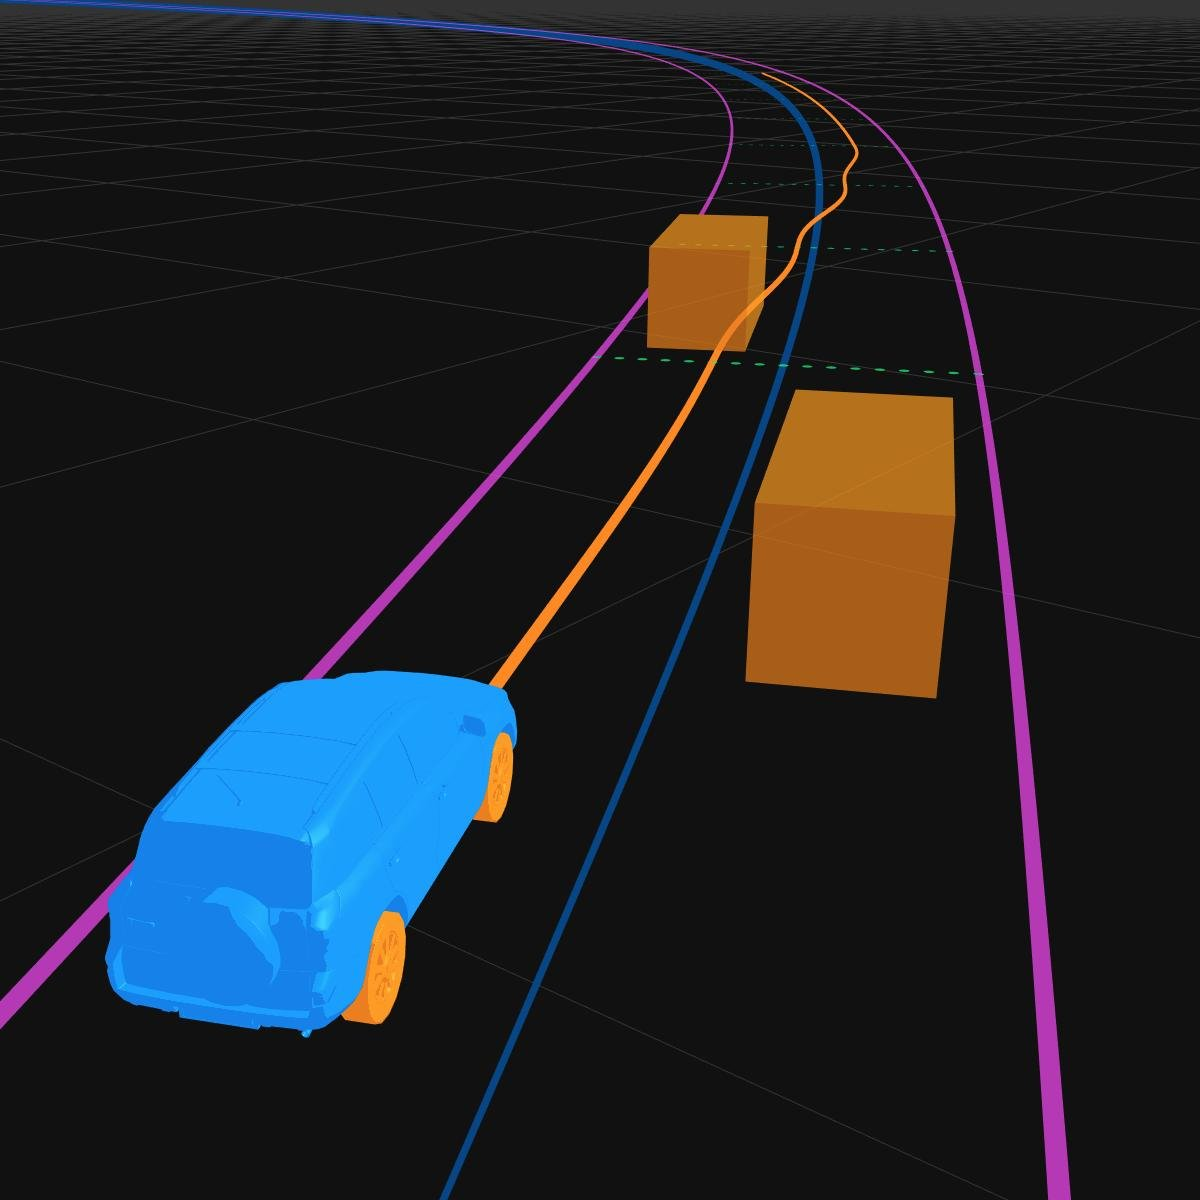
\includegraphics[width=\textwidth,height=4.6cm,keepaspectratio]{scenario3route_bloquee.jpg}
    \caption{Scénario 3 : route bloquée}
  \end{subfigure}\hfill
  \begin{subfigure}[t]{0.48\textwidth}
    \centering
    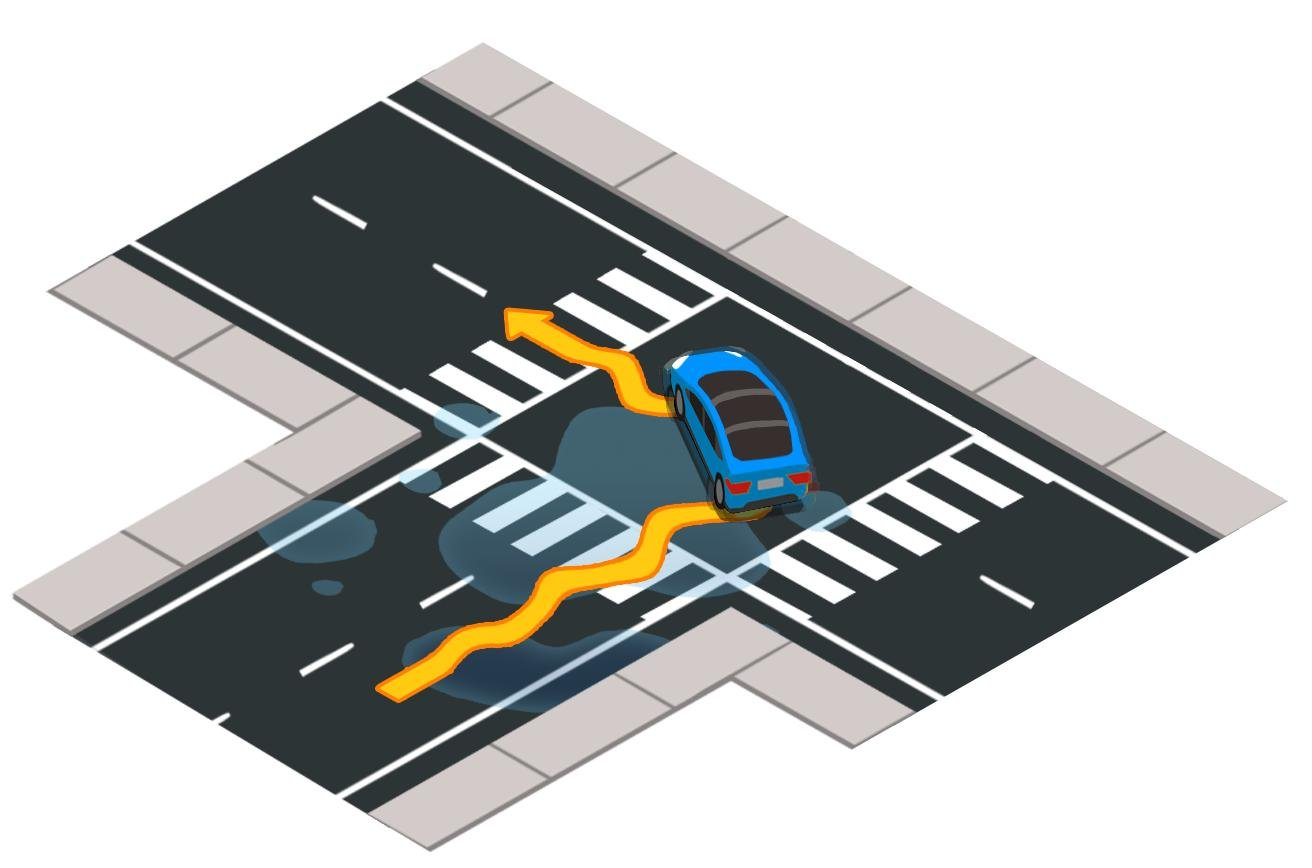
\includegraphics[width=\textwidth,height=4.6cm,keepaspectratio]{scenario4contournement.jpg}
    \caption{Scénario 4 : contournement}
  \end{subfigure}
  \caption{Scénarios de démonstration (illustrations externes)}
  \label{fig:scenarios}
\end{figure}

\begin{itemize}
  \item \textbf{Scénario 1 : route libre (cas nominal)}\\
  Aucun obstacle ne se trouve sur l'itinéraire. Le véhicule suit le chemin calculé par Dijkstra jusqu'à sa destination.
  \item \textbf{Scénario 2 : présence d'un piéton}\\
  Un objet classé \og personne \fg{} se trouve sur l'itinéraire, à moins de 35~m. Le véhicule s'arrête, attend que la personne traverse, puis repart sur le même trajet.
  \item \textbf{Scénario 3 : route bloquée}\\
  Un objet classé \og voiture \fg{}, \og bus \fg{} ou \og camion \fg{} occupe le tronçon. Celui-ci est marqué comme bloqué dans le graphe, et Dijkstra recherche un autre chemin.
  \item \textbf{Scénario 4 : contournement}\\
  Un nouveau chemin existe. Le véhicule change de rue, ou fait demi-tour si nécessaire, puis reprend sa progression vers la destination.
\end{itemize}

Deux cas particuliers sont également prévus. Si le score de confiance est trop faible, la classe devient \og Inconnu \fg{} et le véhicule effectue un arrêt prudent. S'il n'existe plus aucun chemin, le véhicule reste arrêté, et l'épisode est déclaré \og bloqué \fg{} au bout de 30 pas.

\section{Diagramme de cas d'utilisation}

Le diagramme de cas d'utilisation du projet \textit{AutoMaze AI} illustre les différentes interactions entre les acteurs et les fonctionnalités principales du système. L'équipe projet intervient sur toute la chaîne de Machine Learning, de la préparation des données à l'évaluation. L'utilisateur de la démonstration peut classer une image ou lancer un épisode de conduite, tandis que l'encadrante et le jury consultent les résultats. Le diagramme met également en évidence le lien d'\textbf{inclusion} entre la démonstration de conduite et la classification d'une image, puisque chaque obstacle rencontré doit être classé.

\begin{figure}[H]
  \centering
  \resizebox{\textwidth}{!}{% Diagramme de cas d'utilisation : acteurs à gauche et à droite, cas d'utilisation dans le système
\begin{tikzpicture}[
    uc/.style={ellipse, draw=accent, fill=accent!7, align=center, font=\footnotesize,
               minimum width=4.1cm, minimum height=0.95cm, inner sep=1pt},
    lien/.style={draw=black!60},
    inclut/.style={draw=black!50, dashed, -{Stealth[length=2mm]}}
  ]
  % Bonhomme : \acteur{nom}{position}{texte}
  \newcommand{\acteur}[3]{
    \begin{scope}[shift={#2}]
      \draw[thick] (0,0.55) circle (0.17);
      \draw[thick] (0,0.38) -- (0,-0.12);
      \draw[thick] (-0.3,0.2) -- (0.3,0.2);
      \draw[thick] (0,-0.12) -- (-0.22,-0.5);
      \draw[thick] (0,-0.12) -- (0.22,-0.5);
      \node[font=\footnotesize, align=center] at (0,-0.85) {#3};
      \coordinate (#1) at (0,0.1);
    \end{scope}
  }

  % Système
  \draw[draw=black!55, rounded corners=4pt] (2.2,0.9) rectangle (11.4,-8.6);
  \node[anchor=north west, font=\small\bfseries] at (2.3,0.85) {Système AutoMaze AI};

  \node[uc] (u1) at (6.8,-0.4) {UC1 Préparer les données};
  \node[uc] (u2) at (6.8,-1.65) {UC2 Entraîner et comparer\\les classifieurs};
  \node[uc] (u3) at (6.8,-2.9) {UC3 Évaluer le modèle final};
  \node[uc] (u4) at (6.8,-4.15) {UC4 Classer une nouvelle image};
  \node[uc] (u5) at (6.8,-5.4) {UC5 Lancer une démonstration\\de conduite};
  \node[uc] (u6) at (6.8,-6.65) {UC6 Comparer les classifieurs\\dans le simulateur};
  \node[uc] (u7) at (6.8,-7.9) {UC7 Consulter les résultats\\et le rapport};

  \acteur{equipe}{(0,-1.6)}{Équipe\\projet}
  \acteur{utilisateur}{(0,-5.6)}{Utilisateur\\de la démo}
  \acteur{encadrant}{(13.6,-3.2)}{Encadrant}
  \acteur{jury}{(13.6,-6.7)}{Jury}

  \foreach \u in {u1,u2,u3,u6} \draw[lien] (equipe) -- (\u.west);
  \foreach \u in {u4,u5} \draw[lien] (utilisateur) -- (\u.west);
  \draw[lien] (encadrant) -- (u7.east);
  \draw[lien] (encadrant) -- (u3.east);
  \draw[lien] (jury) -- (u7.east);
  \draw[lien] (jury) -- (u5.east);

  % Le cas UC5 inclut la classification d'une image
  \draw[inclut] (u5.north east) to[bend right=30] node[right, font=\scriptsize, text=black!60] {« inclut »} (u4.south east);
\end{tikzpicture}
}
  \caption{Diagramme de cas d'utilisation}
\end{figure}

\section{Diagramme d'activité}

Le diagramme d'activité décrit le déroulement d'un \textbf{épisode de conduite}, depuis le calcul de l'itinéraire jusqu'à l'arrivée. À chaque pas, le véhicule avance puis vérifie s'il a atteint sa destination. Lorsqu'un obstacle se trouve à moins de 35~m, son image est transmise au modèle, et la classe prédite détermine l'action à appliquer. Les coûts des tronçons sont alors mis à jour, et le trajet est recalculé. Ce diagramme met en évidence la coordination entre la perception, la décision et la planification.

\begin{figure}[H]
  \centering
  \resizebox{0.95\textwidth}{!}{% Diagramme d'activité : déroulement d'un épisode de conduite dans le simulateur
\begin{tikzpicture}[
    node distance=0.42cm,
    act/.style={draw=accent, fill=accent!7, rounded corners=6pt, align=center, font=\footnotesize,
                text width=5.4cm, minimum height=0.75cm},
    choix/.style={diamond, draw=black!60, fill=white, aspect=2.4, align=center, font=\scriptsize,
                  inner sep=1pt, text width=2.2cm},
    fleche/.style={-{Stealth[length=2mm]}, draw=black!65, thick}
  ]
  \node[circle, fill=black, minimum size=0.35cm] (debut) {};
  \node[act, below=of debut] (route) {Calculer l'itinéraire avec Dijkstra};
  \node[act, below=of route] (avance) {Avancer d'un pas sur l'itinéraire};
  \node[choix, below=of avance] (arrive) {Destination atteinte ?};
  \node[choix, below=0.5cm of arrive] (obstacle) {Obstacle à moins de 35~m ?};
  \node[act, below=0.5cm of obstacle] (image) {Recevoir l'image de l'obstacle (caméra virtuelle)};
  \node[act, below=of image] (classe) {Classer l'image : classe et score};
  \node[choix, below=of classe] (seuil) {Score au-dessus du seuil ?};
  \node[act, below=0.5cm of seuil] (decision) {Choisir l'action selon la classe prédite};
  \node[act, below=of decision] (couts) {Mettre à jour les coûts des tronçons et recalculer le trajet};
  \node[choix, below=of couts] (chemin) {Un chemin existe ?};

  \node[act, right=1.3cm of seuil] (inconnu) {« Inconnu » : arrêt prudent};
  \node[act, left=1.3cm of chemin] (attente) {Attendre (au plus 30 pas), puis épisode « bloqué »};
  \node[circle, draw=black, thick, minimum size=0.45cm, right=1.3cm of arrive] (fin) {};
  \node[circle, fill=black, minimum size=0.25cm] at (fin) {};

  \draw[fleche] (debut) -- (route);
  \draw[fleche] (route) -- (avance);
  \draw[fleche] (avance) -- (arrive);
  \draw[fleche] (arrive) -- node[above, font=\scriptsize] {oui} (fin);
  \draw[fleche] (arrive) -- node[right, font=\scriptsize] {non} (obstacle);
  \draw[fleche] (obstacle) -- node[right, font=\scriptsize] {oui} (image);
  \draw[fleche] (obstacle.west) -- ++(-1.2,0) node[above, font=\scriptsize, pos=0.4] {non} |- (avance.west);
  \draw[fleche] (image) -- (classe);
  \draw[fleche] (classe) -- (seuil);
  \draw[fleche] (seuil) -- node[right, font=\scriptsize] {oui} (decision);
  \draw[fleche] (seuil) -- node[above, font=\scriptsize] {non} (inconnu);
  \draw[fleche] (inconnu) |- (couts);
  \draw[fleche] (decision) -- (couts);
  \draw[fleche] (couts) -- (chemin);
  \draw[fleche] (chemin.east) -- ++(3.4,0) node[above, font=\scriptsize, pos=0.25] {oui} |- (avance.east);
  \draw[fleche] (chemin) -- node[above, font=\scriptsize] {non} (attente);
\end{tikzpicture}
}
  \caption{Diagramme d'activité d'un épisode de conduite}
\end{figure}

\section{Diagramme de séquence}

Le diagramme de séquence décrit les échanges entre les modules lorsque le véhicule rencontre un obstacle. Le moteur de simulation demande l'image de l'obstacle à la caméra virtuelle, puis la transmet au classifieur, qui renvoie la classe, le score et les six probabilités. La classe prédite et la position de l'obstacle sont ensuite envoyées au système de décision, qui modifie le graphe, avant que le planificateur ne recalcule le trajet. Il est important de noter que la \textbf{vraie classe de l'objet n'apparaît dans aucun message} : le système de décision ne reçoit que la classe prédite.

\begin{figure}[H]
  \centering
  \resizebox{\textwidth}{!}{% Diagramme de séquence : traitement d'un obstacle détecté par le véhicule
\begin{tikzpicture}[
    tete/.style={draw=accent, fill=accent!7, rounded corners=2pt, font=\footnotesize, align=center,
                 minimum width=2.15cm, minimum height=0.8cm},
    msg/.style={-{Stealth[length=2mm]}, draw=black!75},
    retour/.style={-{Stealth[length=2mm]}, draw=black!60, dashed},
    texte/.style={font=\scriptsize, above, align=center}
  ]
  % Lignes de vie : nom, abscisse
  \foreach \nom/\x/\titre in {moteur/0/Moteur\\de simulation, camera/2.6/Caméra\\virtuelle, modele/5.2/Classifieur\\(modèle ML),
                              decision/7.8/Système\\de décision, plan/10.4/Planificateur\\(Dijkstra), vehicule/13/Contrôleur\\du véhicule} {
    \node[tete] (\nom) at (\x,0) {\titre};
    \draw[black!40, dashed] (\x,-0.45) -- (\x,-9.4);
  }

  \draw[msg] (0,-1.2) -- node[texte] {image(obstacle)} (2.6,-1.2);
  \draw[retour] (2.6,-1.8) -- node[texte] {image RGB} (0,-1.8);
  \draw[msg] (0,-2.6) -- node[texte, pos=0.5] {predict(image)} (5.2,-2.6);
  \draw[retour] (5.2,-3.3) -- node[texte, pos=0.5] {classe, score, 6 probabilités} (0,-3.3);
  \draw[msg] (0,-4.1) -- node[texte, pos=0.62] {classe prédite + position de l'obstacle} (7.8,-4.1);
  \draw[msg] (7.8,-4.9) -- node[texte] {bloquer ou pénaliser\\le tronçon} (10.4,-4.9);
  \draw[msg] (10.4,-5.9) -- ++(0.55,0) -- ++(0,-0.45) -- ++(-0.55,0);
  \node[font=\scriptsize, anchor=west, align=left] at (11.05,-6.1) {recalcul\\du trajet};
  \draw[retour] (10.4,-6.9) -- node[texte] {nouvel itinéraire} (7.8,-6.9);
  \draw[msg] (7.8,-7.7) -- node[texte, pos=0.5] {action : arrêter, ralentir, contourner} (13,-7.7);
  \draw[retour] (13,-8.6) -- node[texte, pos=0.5] {nouvelle position du véhicule} (0,-8.6);

  % Activation du classifieur
  \fill[accent!25] (5.1,-2.6) rectangle (5.3,-3.3);
\end{tikzpicture}
}
  \caption{Diagramme de séquence du traitement d'un obstacle}
\end{figure}

\section{Diagramme de composants}

Le diagramme de composants présente l'organisation logicielle du projet. La chaîne de Machine Learning, réalisée dans les notebooks, produit les poids du modèle et le fichier \texttt{metadata.json}. Le simulateur charge ces fichiers à travers son module de perception, et les différents modules communiquent grâce aux contrats partagés définis dans \texttt{contracts.py}.

\begin{figure}[H]
  \centering
  \resizebox{\textwidth}{!}{% Diagramme de composants : modules logiciels et fichiers qui les relient
\begin{tikzpicture}[
    comp/.style={draw=black!60, fill=white, rounded corners=2pt, align=left, font=\footnotesize,
                 text width=3.5cm, minimum height=1.25cm, inner sep=4pt},
    fichier/.style={draw=accent, fill=accent!7, align=center, font=\scriptsize, text width=2.6cm,
                    minimum height=0.8cm},
    zone/.style={draw=black!40, fill=black!3, rounded corners=4pt},
    lien/.style={-{Stealth[length=2mm]}, draw=black!65, thick}
  ]
  % Icône de composant UML (deux petits rectangles)
  \newcommand{\icone}[1]{
    \draw[black!55] ($(#1.north east)+(-0.45,-0.12)$) rectangle ++(0.3,-0.36);
    \draw[black!55, fill=white] ($(#1.north east)+(-0.52,-0.18)$) rectangle ++(0.14,-0.08);
    \draw[black!55, fill=white] ($(#1.north east)+(-0.52,-0.32)$) rectangle ++(0.14,-0.08);
  }

  \draw[zone] (-0.3,0.9) rectangle (4.4,-5.5);
  \node[anchor=north west, font=\small\bfseries] at (-0.2,0.85) {Chaîne ML (notebooks)};
  \draw[zone] (7.6,0.9) rectangle (16.3,-5.5);
  \node[anchor=north west, font=\small\bfseries] at (7.7,0.85) {Simulateur (\texttt{simulator/})};

  \node[comp] (donnees) at (2.05,-0.6) {\textbf{Données}\\Notebooks 01 et 02};
  \node[comp] (modeles) at (2.05,-2.35) {\textbf{Modèles}\\Notebook 03 (et 04)};
  \node[comp] (eval) at (2.05,-4.1) {\textbf{Évaluation}\\Notebook 05};

  \node[fichier] (meta) at (6,-2.35) {\texttt{models/}\\poids et \texttt{metadata.json}};
  \node[fichier] (contrat) at (12,-4.85) {\texttt{contracts.py}\\Prediction, Obstacle, Action};

  \node[comp] (perception) at (9.8,-0.6) {\textbf{Perception}\\Classifieurs, seuil, caméra virtuelle};
  \node[comp] (monde) at (14.2,-0.6) {\textbf{Monde}\\Carte OSM, obstacles, Dijkstra, décisions};
  \node[comp] (moteur) at (9.8,-2.6) {\textbf{Moteur}\\\texttt{engine.py} : épisodes};
  \node[comp] (interface) at (14.2,-2.6) {\textbf{Interface}\\Vues 2D et 3D, HUD};

  \foreach \c in {donnees,modeles,eval,perception,monde,moteur,interface} \icone{\c};

  \draw[lien] (donnees) -- (modeles);
  \draw[lien] (modeles) -- (eval);
  \draw[lien] (modeles.east) -- (meta.west);
  \draw[lien] (meta.north) |- (perception.west);
  \draw[lien] (moteur) -- (perception);
  \draw[lien] (moteur.north east) -- (monde.south west);
  \draw[lien] (interface) -- (moteur);
  % Perception et Monde dépendent de contracts.py : liens par le couloir central, sans traverser les autres modules
  \draw[black!65, thick, dashed] (perception.east) -- (monde.west);
  \fill[black!65] (12,-0.6) circle (1.6pt);
  \draw[lien, dashed] (12,-0.6) -- (contrat.north);
\end{tikzpicture}
}
  \caption{Diagramme de composants}
\end{figure}

\section{Description des interactions entre modules}

\begin{table}[H]
\centering
\small
\caption{Interactions entre les modules du système}
\begin{tabularx}{\textwidth}{>{\raggedright\arraybackslash}p{2.7cm}>{\raggedright\arraybackslash}p{2.7cm}Y}
  \toprule
  \entete \textbf{De} & \textbf{Vers} & \textbf{Information échangée} \\
  \midrule
  Notebooks & Simulateur & Poids du modèle et \texttt{metadata.json} : classes, taille d'entrée, ordre des couleurs, normalisation et seuil \\
  Moteur & Caméra virtuelle & Obstacle rencontré, et en retour une image RGB \\
  Moteur & Classifieur & Image RGB, et en retour une prédiction : classe, score, 6 probabilités et temps de calcul \\
  Moteur & Décision & Classe prédite et tronçon de l'obstacle, et en retour l'action à appliquer \\
  Décision & Planificateur & Tronçons bloqués ou pénalisés, et en retour un nouvel itinéraire \\
  Moteur & Contrôleur & Itinéraire, attente ou ralentissement, et en retour la position du véhicule \\
  Moteur & Interface & État de l'épisode, dernière image, prédiction et décision \\
  \bottomrule
\end{tabularx}
\end{table}

\section{Conclusion}

Ce chapitre a permis de formaliser le \textbf{fonctionnement attendu du système AutoMaze AI} à travers l'identification des acteurs, la description des cas d'utilisation et des scénarios de démonstration, ainsi que plusieurs diagrammes UML. Ces représentations ont contribué à clarifier les échanges entre la perception, la décision et la planification, tout en garantissant que les décisions du véhicule reposent uniquement sur les prédictions du modèle. Elles constituent une base solide pour le chapitre suivant, consacré à l'étude et à la préparation des données.

\chapter{Étude et préparation des données}
\label{chap:donnees}

\section{Introduction}

La qualité d'un modèle de Machine Learning dépend en grande partie des données sur lesquelles il est entraîné. Avant tout apprentissage, il est donc indispensable de choisir un \textbf{jeu de données adapté}, d'en comprendre la composition et de le préparer avec rigueur. Ce chapitre présente l'étude des datasets disponibles, la justification de notre choix, l'analyse quantitative et qualitative des données retenues, puis les différentes étapes de préparation : nettoyage, redimensionnement, normalisation et séparation en jeux d'entraînement, de validation et de test.

\section{Étude des datasets disponibles}

Plusieurs jeux de données publics ont été étudiés afin de trouver celui qui répond le mieux aux besoins du projet.

\begin{table}[H]
\centering
\small
\caption{Comparaison des datasets étudiés}
\begin{tabularx}{\textwidth}{>{\raggedright\arraybackslash}p{3.2cm}>{\raggedright\arraybackslash}p{2.2cm}YY}
  \toprule
  \entete \textbf{Dataset} & \textbf{Classes couvertes} & \textbf{Atouts} & \textbf{Limites} \\
  \midrule
  \href{https://cocodataset.org/\#download}{COCO 2017} & Les 6 & Photos réelles, une boîte annotée par objet & Fort déséquilibre, nombreux petits objets, recadrages à réaliser \\
  CIFAR-10 et CIFAR-100 & Les 6, en combinant les deux & Téléchargement simple, images déjà centrées & Images de 32~×~32~px seulement, peu de scènes routières \\
  Pascal VOC 2012 & 5 sur 6 & Annotations soignées, taille raisonnable & Absence de la classe camion \\
  Jeux Kaggle \og véhicules \fg{} & Variable & Prêts à l'emploi & Qualité et licences inégales, souvent sans personne ni vélo \\
  \bottomrule
\end{tabularx}
\end{table}

\section{Comparaison et justification du dataset retenu}

Le descriptif du projet laisse le choix du jeu de données à l'équipe, en demandant seulement qu'il contienne des images d'objets routiers. Pour départager les options étudiées, nous avons défini cinq critères, directement liés aux besoins du projet :

\begin{itemize}
  \item \textbf{Couverture des classes}\\
  Le dataset doit contenir les six classes retenues, sans devoir en abandonner une.
  \item \textbf{Réalisme des images}\\
  Les photos doivent montrer des objets dans des situations réelles et variées, proches de ce que verrait un véhicule.
  \item \textbf{Résolution suffisante}\\
  Les objets doivent rester reconnaissables une fois recadrés, ce qui exclut les images trop petites.
  \item \textbf{Annotations par objet}\\
  Chaque objet doit être localisé par une boîte, afin de pouvoir le découper automatiquement.
  \item \textbf{Licence et documentation}\\
  Le dataset doit être documenté, cité dans la littérature et utilisable dans un cadre scolaire.
\end{itemize}

\begin{table}[H]
\centering
\small
\caption{Comparaison des datasets selon nos critères}
\begin{tabularx}{\textwidth}{>{\raggedright\arraybackslash}p{3.1cm}YYYY}
  \toprule
  \entete \textbf{Critère} & \textbf{COCO 2017} & \textbf{CIFAR-10/100} & \textbf{Pascal VOC} & \textbf{Kaggle} \\
  \midrule
  Couverture des 6 classes & Oui & Oui, en combinant les deux & Non (5 sur 6) & Variable \\
  Réalisme des images & Oui, scènes réelles variées & Faible, objets isolés & Oui & Variable \\
  Résolution & Médiane de 640~×~480~px & 32~×~32~px & Correcte & Variable \\
  Annotations par objet & Oui, boîtes englobantes & Non, une étiquette par image & Oui & Variable \\
  Documentation et licence & Article de référence, licences précisées & Documenté & Documenté & Inégales \\
  \bottomrule
\end{tabularx}
\end{table}

Au regard de ces critères, nous avons retenu \textbf{COCO 2017}, sous réserve de la validation de notre encadrante. Il s'agit du seul dataset étudié qui remplit l'ensemble des critères : il couvre nos six classes avec de \textbf{vraies photos}, prises dans des conditions variées, et fournit des \textbf{annotations de référence} pour chaque objet. De plus, il n'est pas nécessaire de télécharger les 18~Go d'images, puisque seules les photos utiles sont récupérées grâce à leur adresse. CIFAR reste notre solution de secours, malgré sa résolution très faible.

\subsection{Source et description du dataset retenu}

\begin{table}[H]
\centering
\small
\caption{Fiche descriptive du dataset COCO 2017}
\begin{tabularx}{\textwidth}{>{\raggedright\arraybackslash}p{3.6cm}Y}
  \toprule
  \entete \textbf{Élément} & \textbf{Description} \\
  \midrule
  Nom & COCO (\textit{Common Objects in Context}), version 2017 \\
  Auteurs & Microsoft et plusieurs équipes universitaires, publication de référence de Lin et al. (2014) \cite{coco} \\
  Source & Site officiel \url{https://cocodataset.org}, rubrique \textit{Download} \\
  Contenu & 80 catégories d'objets du quotidien, dont nos six classes \\
  Volume & 118~287 images d'entraînement (\texttt{train2017}) et 5~000 images de validation (\texttt{val2017}) \\
  Annotations & Fichiers JSON : catégorie, boîte englobante et indicateur de foule pour chaque objet \\
  Licences & Annotations sous licence CC~BY~4.0, images sous la licence Flickr choisie par chaque auteur \\
  Utilisation dans le projet & \texttt{train2017} pour constituer nos jeux d'entraînement, de validation et de test, et \texttt{val2017} réservé aux tests sur de nouvelles images \\
  \bottomrule
\end{tabularx}
\end{table}

Concrètement, nous téléchargeons d'abord le fichier d'annotations de \texttt{train2017}, qui décrit chaque objet sans contenir les images. Nous sélectionnons ensuite les objets utiles, puis nous téléchargeons uniquement les photos correspondantes à partir de leur adresse. Les licences imposent de citer COCO et de ne pas redistribuer les images : celles-ci restent donc hors du dépôt Git, qui ne conserve que de petites vignettes dans les figures.

\section{Présentation des classes}

Les six classes retenues correspondent aux usagers de la route que le véhicule doit savoir reconnaître :

\begin{itemize}
  \item \textbf{Personne (\texttt{person})}\\
  Il s'agit de l'usager le plus vulnérable. Une erreur sur cette classe est donc la plus grave pour un véhicule.
  \item \textbf{Vélo (\texttt{bicycle})}\\
  Usager lent et fragile, souvent accompagné d'une personne. Il faut noter que COCO annote le vélo et non le cycliste.
  \item \textbf{Voiture (\texttt{car})}\\
  Usager le plus fréquent, souvent à l'arrêt sur la chaussée.
  \item \textbf{Moto (\texttt{motorcycle})}\\
  Véhicule léger et rapide, visuellement proche du vélo.
  \item \textbf{Bus (\texttt{bus})}\\
  Grand véhicule qui masque une partie de la visibilité.
  \item \textbf{Camion (\texttt{truck})}\\
  Grand véhicule. COCO range également dans cette classe des pick-ups et des camionnettes.
\end{itemize}

L'ordre des classes (personne, vélo, voiture, moto, bus, camion) est fixé une fois pour toutes, car il correspond aux sorties du modèle et à ce qu'attend le simulateur.

\begin{figure}[H]
  \centering
  \begin{subfigure}[t]{0.155\textwidth}\centering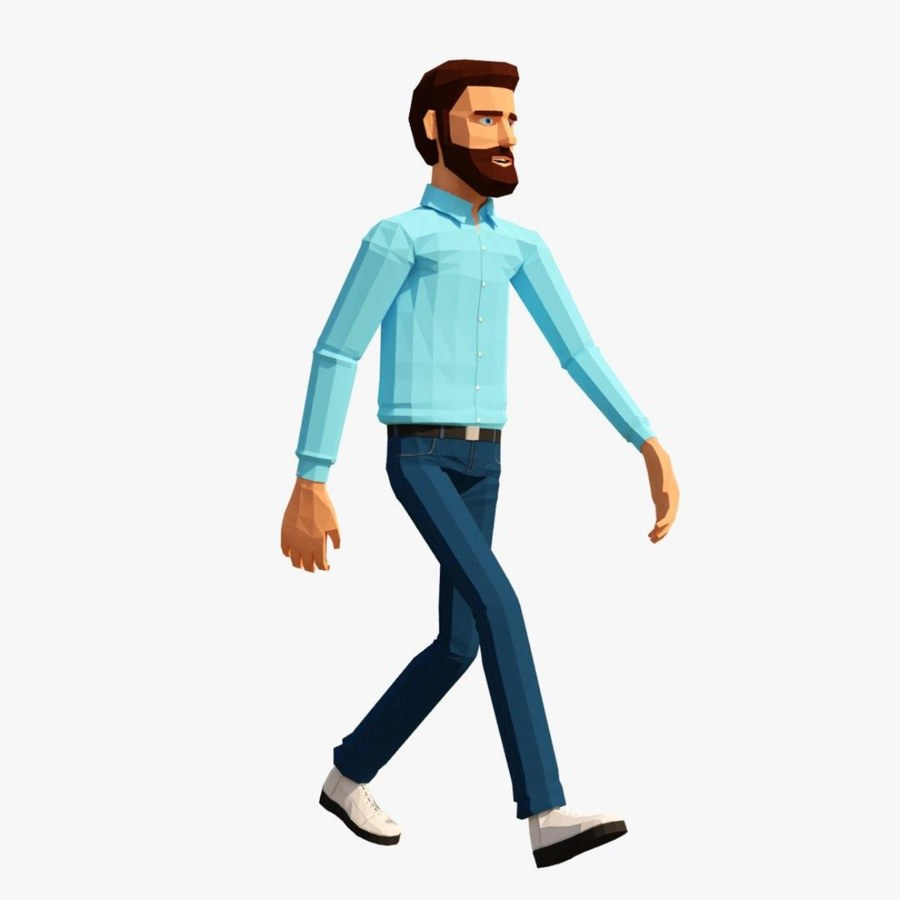
\includegraphics[width=\textwidth,height=2.6cm,keepaspectratio]{obj_person.jpg}\caption*{Personne}\end{subfigure}\hfill
  \begin{subfigure}[t]{0.155\textwidth}\centering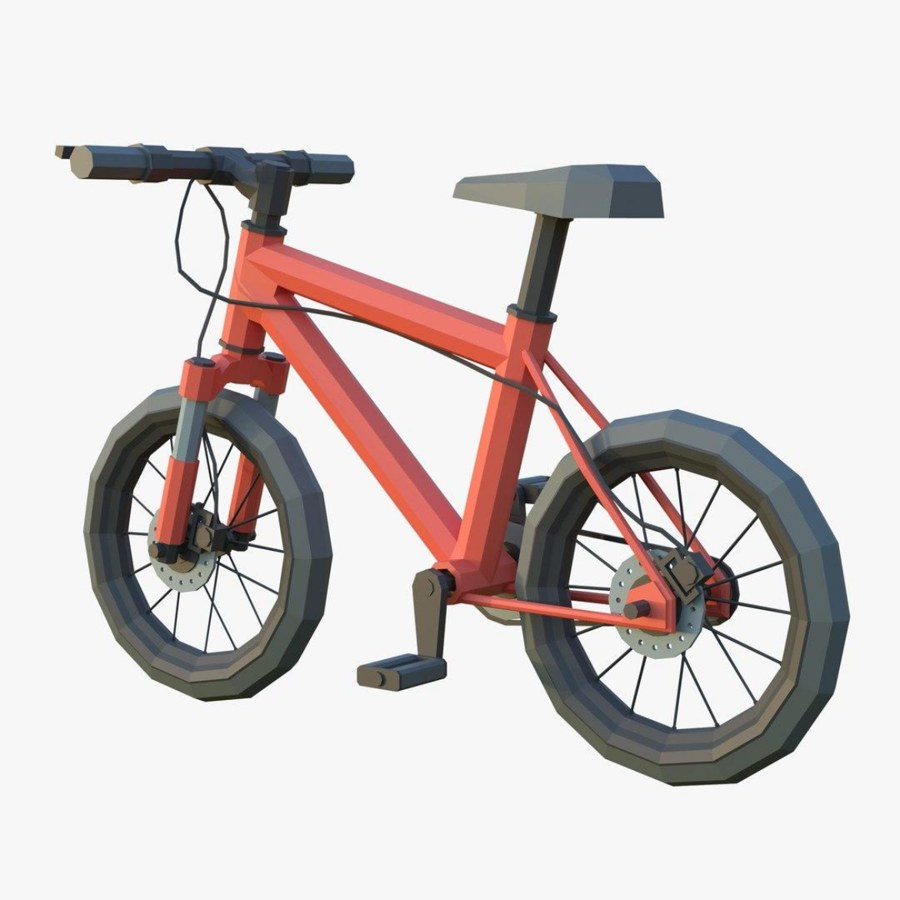
\includegraphics[width=\textwidth,height=2.6cm,keepaspectratio]{obj_velo.jpg}\caption*{Vélo}\end{subfigure}\hfill
  \begin{subfigure}[t]{0.155\textwidth}\centering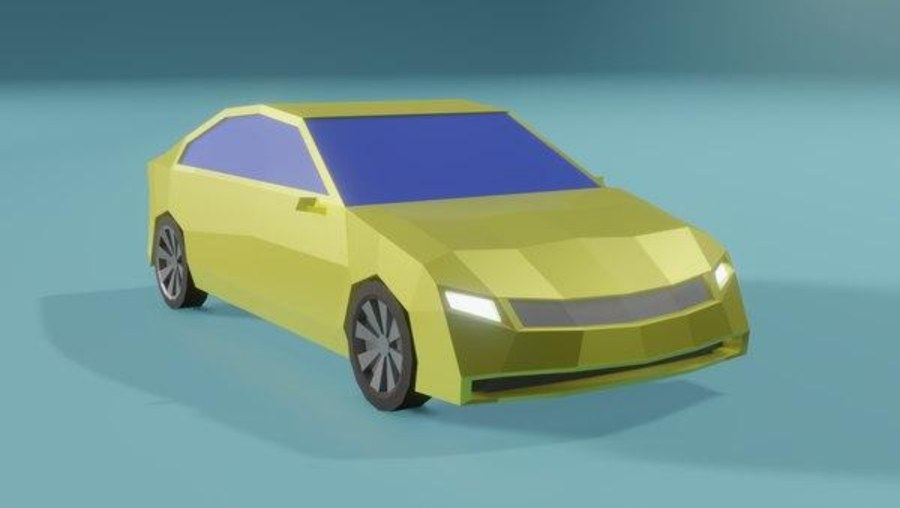
\includegraphics[width=\textwidth,height=2.6cm,keepaspectratio]{obj_voiture.jpg}\caption*{Voiture}\end{subfigure}\hfill
  \begin{subfigure}[t]{0.155\textwidth}\centering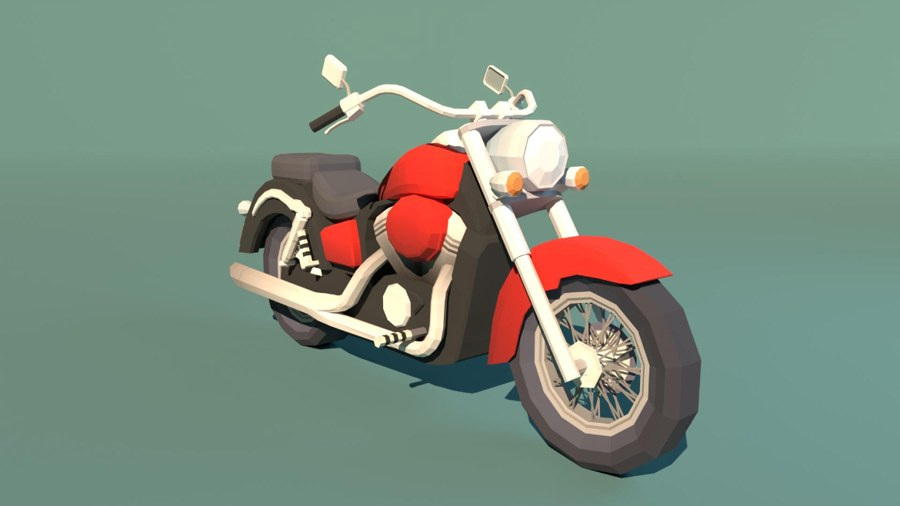
\includegraphics[width=\textwidth,height=2.6cm,keepaspectratio]{obj_moto.jpg}\caption*{Moto}\end{subfigure}\hfill
  \begin{subfigure}[t]{0.155\textwidth}\centering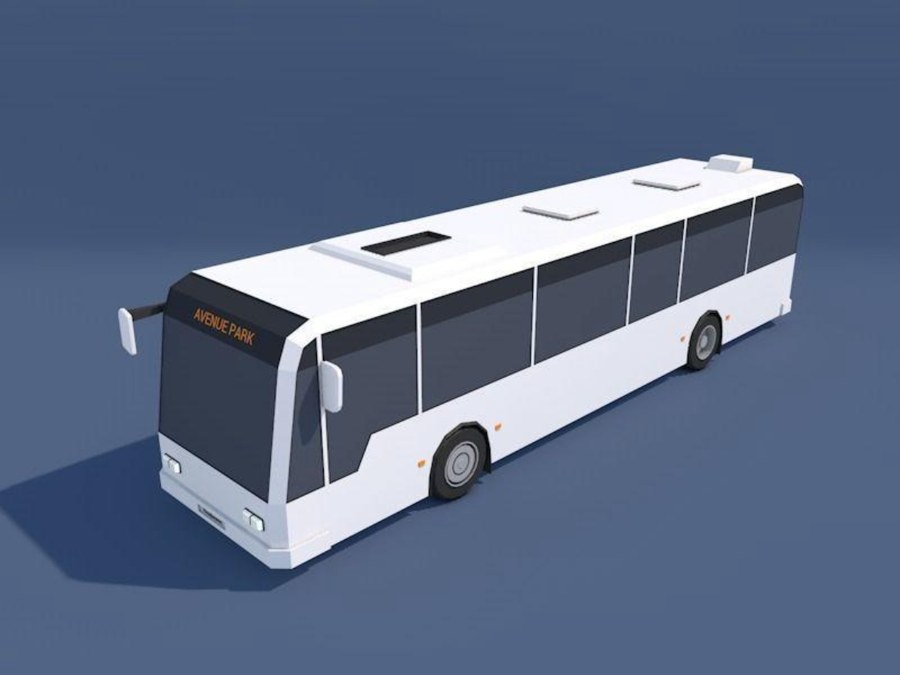
\includegraphics[width=\textwidth,height=2.6cm,keepaspectratio]{obj_bus.jpg}\caption*{Bus}\end{subfigure}\hfill
  \begin{subfigure}[t]{0.155\textwidth}\centering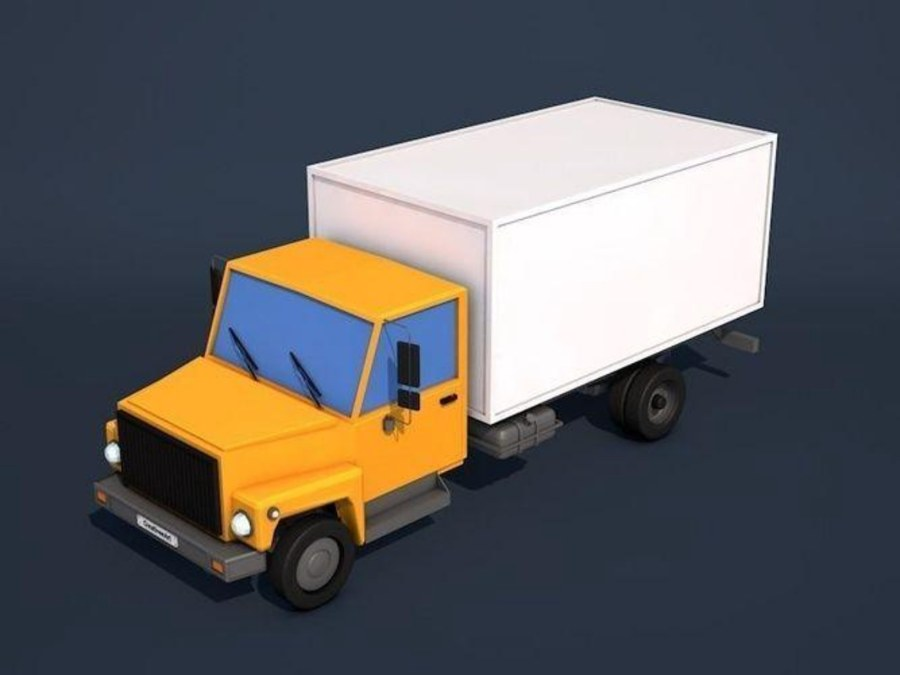
\includegraphics[width=\textwidth,height=2.6cm,keepaspectratio]{obj_camion.jpg}\caption*{Camion}\end{subfigure}
  \caption{Illustration des six classes par des modèles 3D (le modèle apprend sur des photos réelles de COCO)}
\end{figure}

\section{Analyse quantitative des données}

L'ensemble \texttt{train2017} de COCO compte \textbf{118~287 images}, dont \textbf{70~082} contiennent au moins un objet de nos classes. La résolution médiane de ces images est de 640~×~480~px.

\begin{table}[H]
\centering
\small
\caption{Nombre d'objets disponibles par classe dans COCO \texttt{train2017}}
\begin{tabular}{lrr}
  \toprule
  \entete \textbf{Classe} & \textbf{Objets annotés} & \textbf{Hors foules, plus petit côté d'au moins 32~px} \\
  \midrule
  Personne & 262~465 & 150~185 \\
  Voiture & 43~867 & 16~799 \\
  Camion & 9~973 & 7~071 \\
  Moto & 8~725 & 6~742 \\
  Vélo & 7~113 & 4~505 \\
  Bus & 6~069 & 5~194 \\
  \bottomrule
\end{tabular}
\end{table}

\begin{figure}[H]
  \centering
  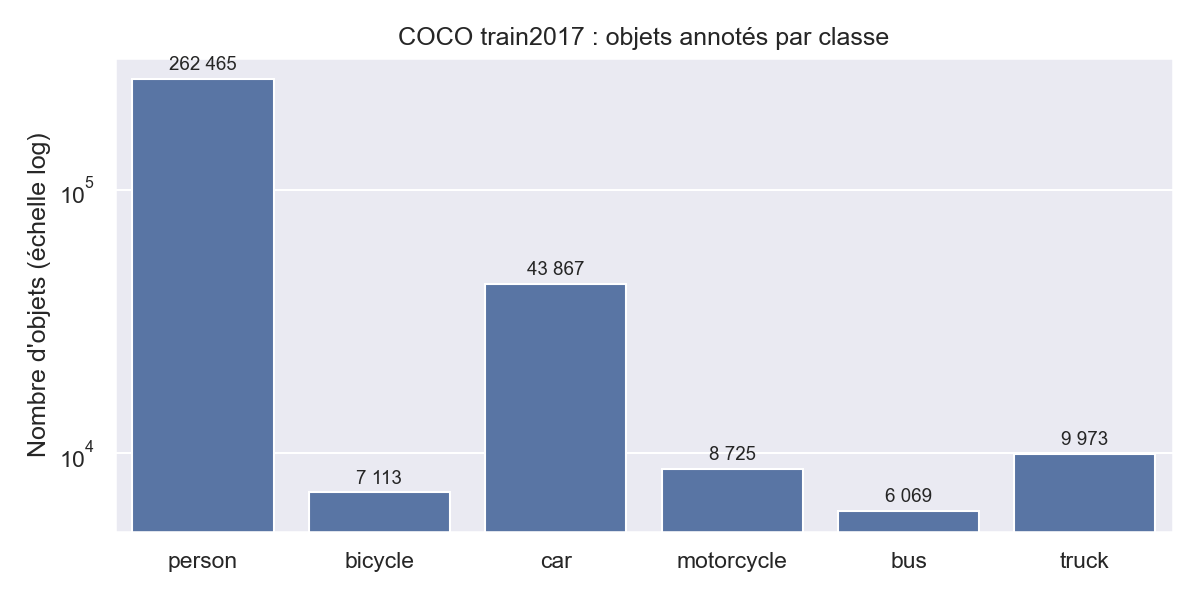
\includegraphics[width=0.66\textwidth]{01_repartition_classes.png}
  \caption{Répartition des objets par classe avant filtrage}
\end{figure}

Ces chiffres mettent en évidence un \textbf{fort déséquilibre} entre les classes : on compte 43,2 personnes pour un bus. Sans précaution, un modèle pourrait obtenir une bonne accuracy en répondant presque toujours \og personne \fg{}. C'est pourquoi nous limitons le nombre d'objets par classe et évaluons les modèles avec le F1 macro.

\section{Analyse qualitative des images}

L'observation d'exemples tirés au hasard a permis de relever plusieurs difficultés :

\begin{itemize}
  \item des objets \textbf{coupés} par le bord de la photo ou \textbf{cachés} par un autre objet ;
  \item des images \textbf{floues} ou très petites, en particulier pour les voitures éloignées ;
  \item \textbf{plusieurs objets} dans un même recadrage, comme un motard sur sa moto ;
  \item une classe \og camion \fg{} \textbf{hétérogène}, qui contient aussi des pick-ups et des camionnettes, proches d'une voiture ;
  \item des photos prises par des particuliers et non depuis un véhicule, ce qui constitue un biais à garder en tête pour un usage routier.
\end{itemize}

\section{Nettoyage des données}

Afin de ne conserver que des exemples exploitables, plusieurs règles de nettoyage ont été appliquées :

\begin{itemize}
  \item \textbf{Exclusion des foules}\\
  Une boîte marquée \texttt{iscrowd} entoure un groupe de personnes et non un seul usager.
  \item \textbf{Exclusion des petits objets}\\
  En dessous de 32~px de côté, l'objet devient trop flou une fois agrandi. À ce seuil, la classe la plus rare conserve 4~505 objets, contre seulement 2~693 avec un seuil de 64~px.
  \item \textbf{Plafond de 2~500 objets par classe}\\
  Ce plafond permet d'équilibrer les classes tout en gardant un entraînement réalisable sans GPU.
  \item \textbf{Contrôle des téléchargements}\\
  Une photo inaccessible est notée sans interrompre la préparation. Sur les 15~000 objets prévus, 14~990 ont été récupérés, 8 téléchargements ayant expiré.
\end{itemize}

\section{Redimensionnement et normalisation}

Chaque objet est découpé dans un \textbf{carré} centré sur sa boîte, avec une marge de 10~\%, puis réduit à \textbf{64~×~64~px}. Le recadrage carré évite de déformer les silhouettes, une personne étant haute et fine alors qu'un bus est large. Lorsque le carré dépasse les bords de la photo, les pixels manquants sont complétés par \textbf{reflet} plutôt que par une bande noire, que le modèle pourrait apprendre à tort.

Chaque canal de couleur est ensuite \textbf{normalisé} à l'aide de la moyenne et de l'écart-type calculés sur le jeu d'entraînement, soit [0,4057 ; 0,3894 ; 0,3748] pour la moyenne et [0,2609 ; 0,2554 ; 0,2571] pour l'écart-type. Le simulateur applique exactement les mêmes valeurs.

\begin{figure}[H]
  \centering
  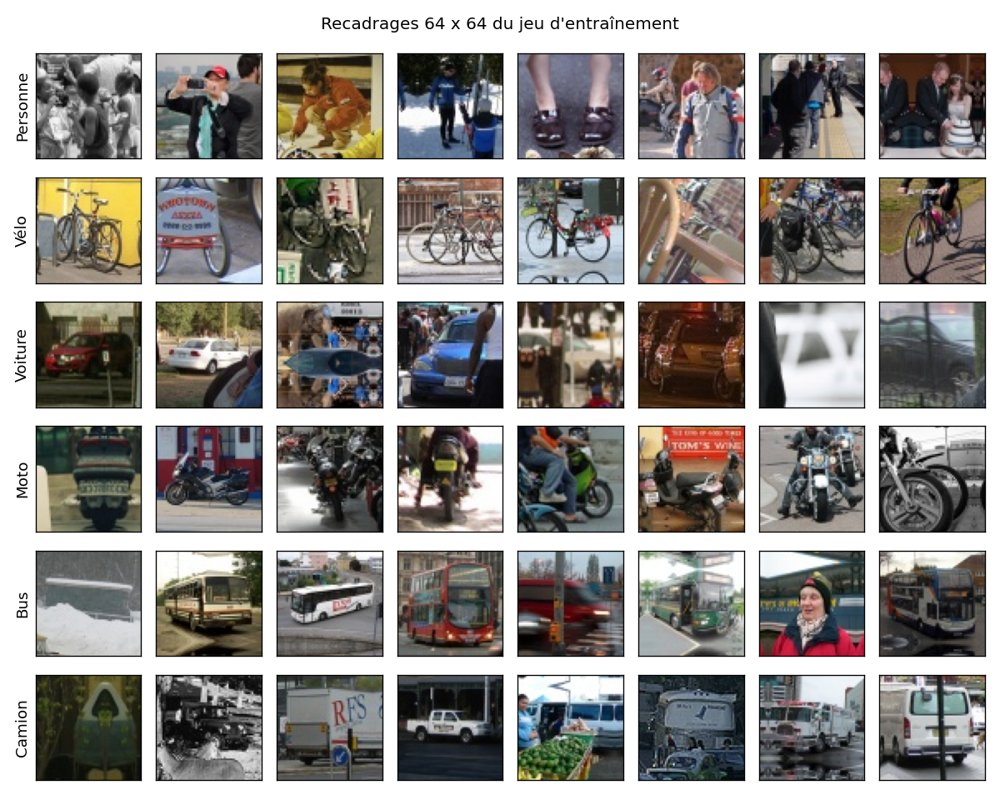
\includegraphics[width=0.58\textwidth]{02_recadrages.jpg}
  \caption{Recadrages de 64~×~64~px du jeu d'entraînement, une ligne par classe}
  \label{fig:recadrages}
\end{figure}

\section{Séparation entraînement, validation et test}

Les données ont été réparties en trois jeux : \textbf{70~\%} pour l'entraînement, \textbf{15~\%} pour la validation et \textbf{15~\%} pour le test.

\begin{table}[H]
\centering
\small
\caption{Répartition des images par classe et par jeu}
\begin{tabular}{lrrr}
  \toprule
  \entete \textbf{Classe} & \textbf{Entraînement} & \textbf{Validation} & \textbf{Test} \\
  \midrule
  Personne & 1~750 & 375 & 375 \\
  Vélo & 1~748 & 373 & 375 \\
  Voiture & 1~750 & 375 & 374 \\
  Moto & 1~750 & 374 & 375 \\
  Bus & 1~748 & 374 & 375 \\
  Camion & 1~749 & 375 & 375 \\
  \bottomrule
\end{tabular}
\end{table}

Le découpage est \textbf{stratifié}, afin de conserver les mêmes proportions de classes dans chaque jeu. Il est également réalisé \textbf{par photo d'origine}, car deux objets d'une même photo partagent le même éclairage et le même décor. Les répartir entre l'entraînement et le test fausserait donc le score. Un contrôle automatique vérifie qu'aucune des 10~672 photos n'apparaît dans deux jeux, et le découpage est enregistré dans un fichier commun afin que toute l'équipe utilise exactement les mêmes données.

\section{Conclusion}

Ce chapitre a permis de justifier le choix de \textbf{COCO 2017} et de décrire précisément les données retenues. L'analyse a mis en évidence un fort déséquilibre entre les classes ainsi que plusieurs difficultés liées à la qualité des images. Les étapes de nettoyage, de recadrage, de normalisation et de découpage par photo garantissent un jeu de données équilibré et une évaluation fiable. Ces données préparées serviront de base au modèle de classification, dont l'intégration dans l'architecture globale est détaillée dans le chapitre suivant.

\chapter{Architecture technique et conception des modules}
\label{chap:architecture}

\section{Introduction}

Après avoir défini les besoins du système et préparé les données, il est désormais essentiel d'aborder l'\textbf{aspect technique} du projet. Ce chapitre a pour objectif de présenter l'architecture globale d'AutoMaze AI, en détaillant le rôle de chaque module ainsi que leurs interactions. Une attention particulière sera accordée à la \textbf{séparation entre la vérité terrain du simulateur et la perception du modèle}, qui garantit que les décisions du véhicule reflètent réellement la qualité de notre classifieur.

\section{Architecture globale d'AutoMaze AI}

L'architecture du projet repose sur un principe simple. Le simulateur connaît la position de chaque objet présent dans son environnement, tandis que le \textbf{modèle de Machine Learning} analyse l'image fournie par la caméra virtuelle et en détermine la nature. Le système associe ensuite la classe prédite à la position connue de l'objet. Le \textbf{planificateur} calcule le chemin vers la destination et le recalcule lorsqu'un obstacle rend le trajet impraticable. Enfin, le \textbf{contrôleur} applique les décisions au véhicule virtuel : continuer, ralentir, s'arrêter ou changer de direction.

\begin{figure}[H]
  \centering
  \resizebox{\textwidth}{!}{% Architecture fonctionnelle globale d'AutoMaze AI (cinq étages, de l'environnement au contrôleur)
\begin{tikzpicture}[
    etage/.style={draw=accent, fill=accent!7, rounded corners=3pt, align=center, font=\footnotesize,
                  text width=12.2cm, minimum height=1.0cm, inner sep=4pt},
    bloc/.style={draw=black!60, fill=white, rounded corners=3pt, align=center, font=\footnotesize,
                 text width=3.6cm, minimum height=1.05cm, inner sep=3pt},
    ml/.style={bloc, draw=accent, fill=accent!18, very thick},
    fleche/.style={-{Stealth[length=2.2mm]}, draw=black!70, thick}
  ]
  \node[etage] (env) at (0,0) {\textbf{1. Environnement de simulation}\\Routes · Véhicule · Objets routiers · Destination};

  \node[bloc] (camera) at (-4.3,-1.75) {\textbf{Caméra virtuelle}\\Image de l'objet};
  \node[ml] (modele) at (-4.3,-3.35) {\textbf{Modèle ML}\\Classification de l'objet};
  \node[bloc] (infos) at (4.3,-2.55) {\textbf{Informations du simulateur}\\Coordonnées et positions des objets};
  \node[bloc] (etat) at (0,-4.75) {\textbf{État des obstacles}\\Position + nature identifiée};

  \node[etage] (fusion) at (0,-6.3) {\textbf{2. Fusion des informations et représentation de l'environnement}\\Association de la classe prédite aux coordonnées de l'objet correspondant};
  \node[etage] (plan) at (0,-7.75) {\textbf{3. Planificateur}\\Graphe · Dijkstra · Recalcul du trajet};
  \node[etage] (decision) at (0,-9.2) {\textbf{4. Système de décision}\\Ralentir · Arrêter · Contourner · Continuer};
  \node[etage] (controle) at (0,-10.65) {\textbf{5. Contrôleur du véhicule}\\Vitesse · Freinage · Direction};
  \node[font=\footnotesize\bfseries, text=integration] (but) at (0,-11.75) {Déplacement autonome jusqu'à la destination};

  \draw[fleche] (env.south -| camera) -- (camera);
  \draw[fleche] (camera) -- (modele);
  \draw[fleche] (env.south -| infos) -- (infos);
  \draw[fleche] (modele.south) |- (etat.west);
  \draw[fleche] (infos.south) |- (etat.east);
  \draw[fleche] (etat) -- (fusion);
  \draw[fleche] (fusion) -- (plan);
  \draw[fleche] (plan) -- (decision);
  \draw[fleche] (decision) -- (controle);
  \draw[fleche] (controle) -- (but);

  % Une décision qui bloque un tronçon relance le planificateur
  \draw[fleche, dashed, draw=accent] (decision.east) -- ++(0.55,0) |- node[pos=0.25, right, font=\scriptsize, align=left, text=accent] {obstacle\\bloquant :\\recalcul} (plan.east);
  % Le véhicule se déplace dans l'environnement : la boucle reprend
  \draw[fleche, draw=integration] (but.west) -- ++(-6.9,0) |- node[pos=0.25, left, font=\scriptsize, text=integration, align=right] {nouvelle\\position} (env.west);

  % Ce que le simulateur ne transmet pas
  \node[font=\scriptsize, text=black!65, align=center, text width=3.8cm] at (4.3,-3.95) {La vraie classe de l'objet n'est jamais transmise à la décision};
\end{tikzpicture}
}
  \caption{Architecture fonctionnelle globale d'AutoMaze AI}
  \label{fig:architecture}
\end{figure}

\section{Environnement de simulation}
\label{sec:environnement}

Notre environnement de simulation reproduit une partie réelle de \textbf{Casablanca}, du Twin Center (Maârif) à la place Mohammed V. Le réseau routier provient d'\textbf{OpenStreetMap} et respecte les sens uniques. Le véhicule circule à 8~m/s, soit environ 29~km/h, et le temps avance par pas d'une seconde. Chaque épisode place six obstacles sur l'itinéraire, et trois vues sont proposées : une carte en 2D, une vue conducteur et une vue en 3D.

Les simulateurs de conduite professionnels offrent des environnements 3D très détaillés, comme l'illustre la figure~\ref{fig:inspiration}. Notre simulateur reste volontairement plus simple, puisqu'il sert uniquement à démontrer l'utilisation du modèle.

\begin{figure}[H]
  \centering
  \begin{subfigure}[t]{0.49\textwidth}
    \centering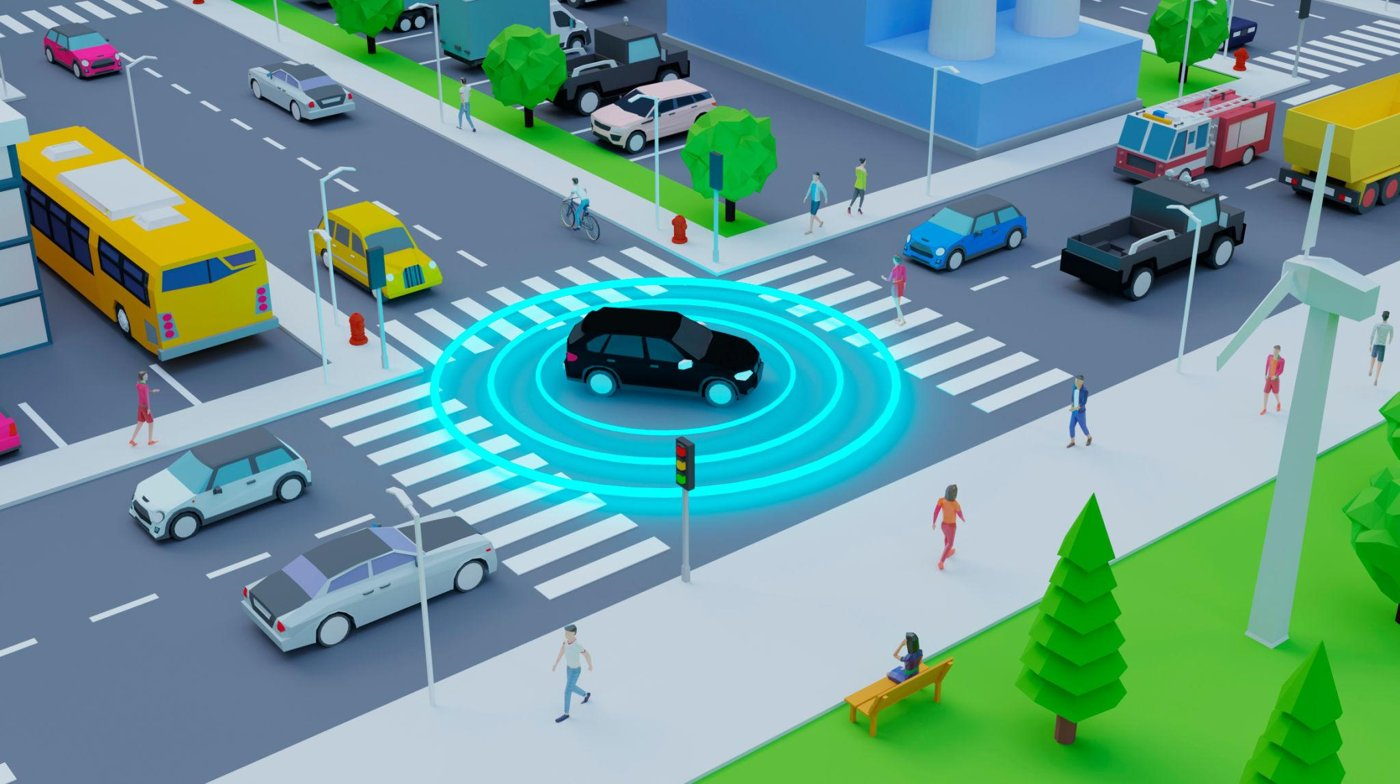
\includegraphics[width=\textwidth]{environnement_vir1.jpg}
  \end{subfigure}\hfill
  \begin{subfigure}[t]{0.49\textwidth}
    \centering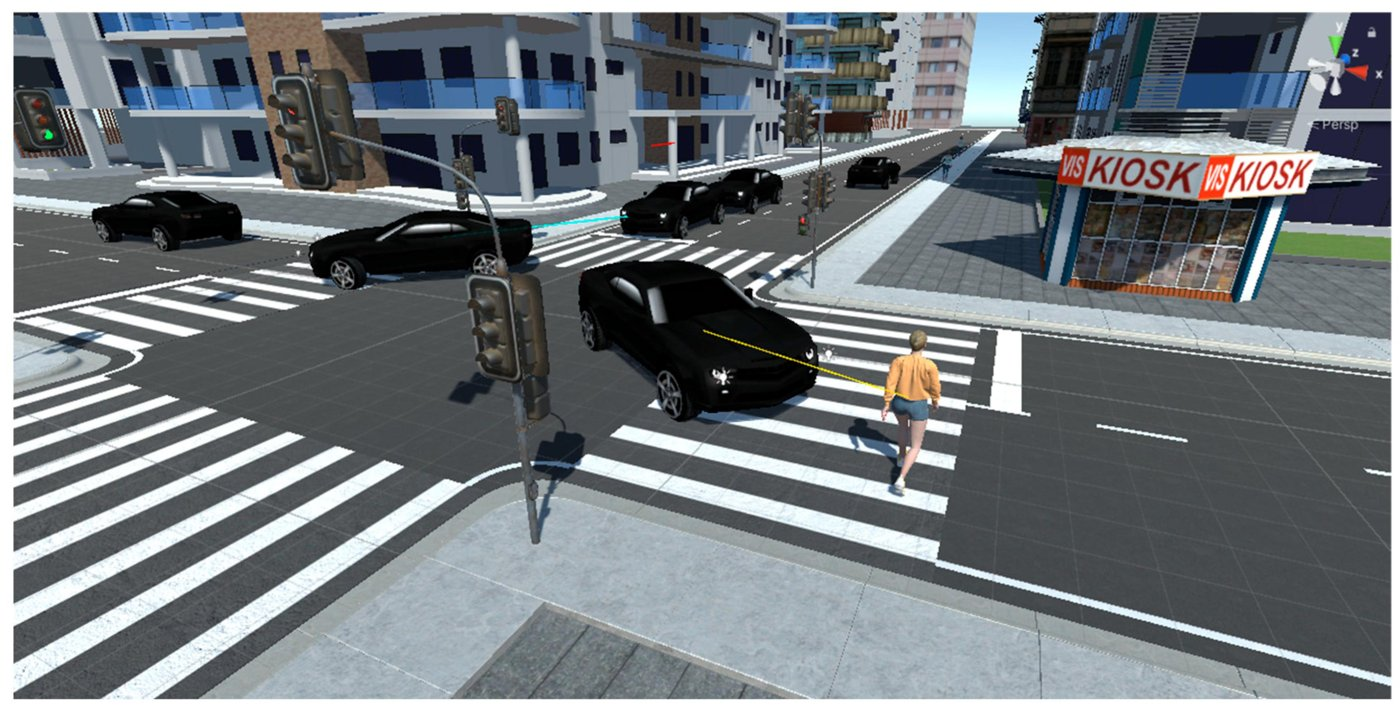
\includegraphics[width=\textwidth]{environnement_vir2.jpg}
  \end{subfigure}
  \caption{Exemples d'environnements virtuels de conduite ayant servi d'inspiration (sources externes)}
  \label{fig:inspiration}
\end{figure}

\begin{figure}[H]
  \centering
  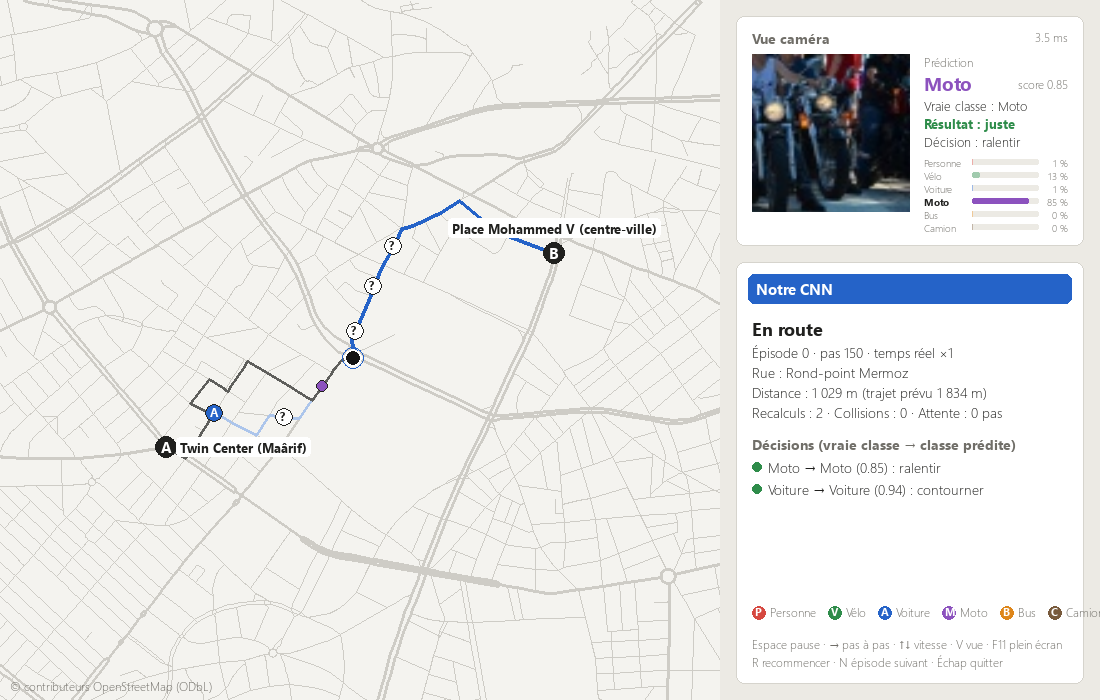
\includegraphics[width=0.82\textwidth]{06_simulateur_carte.png}
  \caption{Notre simulateur en vue carte : itinéraire, obstacles et dernière prédiction (carte © contributeurs OpenStreetMap)}
  \label{fig:notre-simulateur}
\end{figure}

\section{Acquisition des images par caméra virtuelle}
\label{sec:camera}

Lorsqu'un obstacle se trouve sur l'itinéraire à moins de 35~m, la \textbf{caméra virtuelle} transmet son image au modèle.

Ce module repose sur un choix de conception important. Si la caméra filmait les objets 3D du simulateur, le modèle recevrait des images de synthèse très différentes des photos sur lesquelles il a appris, et ses performances chuteraient. La caméra fournit donc une \textbf{vraie photo} de la classe de l'obstacle, tirée du jeu de test, que le modèle n'a jamais vue. Les modèles 3D servent uniquement à l'affichage. De plus, une même graine aléatoire donne les mêmes images à tous les classifieurs comparés, tandis que les images changent d'un épisode à l'autre.

\subsection{Association d'une image à chaque objet}

L'association entre un objet du simulateur et l'image transmise au modèle se déroule en quatre étapes :

\begin{enumerate}
  \item \textbf{Création de l'obstacle}\\
  Au début de chaque épisode, le simulateur place six obstacles sur l'itinéraire. Chacun reçoit une position (un tronçon de rue et une distance sur ce tronçon) ainsi qu'une vraie classe, tirée au hasard parmi les six.
  \item \textbf{Choix de l'image}\\
  Lorsque le véhicule arrive à moins de 35~m de l'obstacle, la caméra virtuelle choisit une image dans le dossier du jeu de test correspondant à sa vraie classe (\texttt{data/crops/test/<classe>/}). Si l'obstacle est un camion, la caméra \og voit \fg{} donc la photo d'un vrai camion que le modèle n'a jamais rencontrée.
  \item \textbf{Tirage reproductible}\\
  Le choix de l'image dépend de la graine de l'expérience, de la position de l'obstacle et du numéro de l'épisode. Ainsi, un même obstacle reçoit toujours la même image, quel que soit le classifieur testé, ce qui garantit une comparaison équitable. L'image est ensuite conservée en mémoire, afin que le véhicule voie la même photo s'il repasse devant l'obstacle.
  \item \textbf{Transmission au modèle}\\
  L'image est transmise au classifieur actif, sans aucune indication sur sa vraie classe. La prédiction obtenue est alors rattachée à l'obstacle d'origine (section~\ref{sec:association}).
\end{enumerate}

La vraie classe sert donc uniquement à choisir ce que la caméra \og voit \fg{}, comme dans la réalité, où un camion présent sur la route apparaît sur l'image de la caméra. Elle n'intervient jamais dans la décision du véhicule, qui repose seulement sur la prédiction du modèle. Si aucune image n'est disponible pour une classe, par exemple avant la préparation des données, le simulateur génère une image de remplacement.

\section{Module de classification par Machine Learning}
\label{sec:module-classification}

Le module de classification reçoit l'image RGB d'un objet, quelle que soit sa taille, et applique lui-même le prétraitement : mise au carré, réduction à 64~×~64~px et normalisation. Il renvoie ensuite :

\begin{itemize}
  \item la \textbf{classe prédite}, parmi les six classes ;
  \item un \textbf{score de confiance}, correspondant au plus grand des six scores ;
  \item les \textbf{six scores}, dont la somme vaut 1 ;
  \item le \textbf{temps de calcul} réellement mesuré.
\end{itemize}

L'affichage prend par exemple la forme \og Image \textrightarrow{} Voiture (92~\%) \fg{}. Ce pourcentage est un exemple d'affichage et non une performance mesurée. Il s'agit d'un score et non d'une probabilité calibrée, ce qui signifie que le modèle n'a pas forcément raison 92 fois sur 100.

Lorsque le score est inférieur à un certain seuil, la classe devient \og Inconnu \fg{} et le véhicule effectue un arrêt prudent. Ce \textbf{seuil} sera choisi sur le jeu de validation, puis enregistré avec le modèle.

Enfin, trois classifieurs respectent la même interface et sont donc interchangeables : un mode \og simulation \fg{}, qui permet de tester la logique sans modèle, notre propre modèle, et un éventuel modèle de référence préentraîné, utilisé uniquement comme point de comparaison si l'encadrante l'accepte.

\section{Module de localisation et association des objets}
\label{sec:association}

Le simulateur décrit chaque obstacle par un identifiant et une position sur la carte, comme le montre l'exemple suivant.

\begin{table}[H]
\centering
\small
\caption{Exemple d'association entre position et classe prédite}
\begin{tabularx}{\textwidth}{>{\raggedright\arraybackslash}p{2cm}>{\raggedright\arraybackslash}p{4.4cm}>{\raggedright\arraybackslash}p{2.6cm}Y}
  \toprule
  \entete \textbf{Identifiant} & \textbf{Position} & \textbf{Classe prédite} & \textbf{Vraie classe (cachée)} \\
  \midrule
  OBJ-01 & Tronçon A \textrightarrow{} B, à 45~m de A & Voiture & Voiture \\
  OBJ-02 & Tronçon C \textrightarrow{} D, à 12~m de C & Personne & Personne \\
  OBJ-03 & Tronçon E \textrightarrow{} F, à 30~m de E & Voiture & Camion \\
  \bottomrule
\end{tabularx}
\end{table}

L'\textbf{association} entre une prédiction et un objet est directe : chaque image est produite pour un obstacle précis, et la prédiction est donc rattachée à l'objet dont elle provient. Ce choix, simple et sûr, est possible car chaque image ne contient qu'un seul objet.

Il est essentiel de bien séparer deux types d'informations :

\begin{itemize}
  \item \textbf{La vérité terrain}\\
  Elle regroupe la vraie classe et la position de l'objet. Elle sert à construire les scénarios, à faire agir l'obstacle selon sa vraie nature (une personne finit de traverser, un camion reste immobile) et à mesurer les erreurs.
  \item \textbf{La perception}\\
  Elle correspond à la classe prédite par notre modèle. C'est la seule information transmise au système de décision. Une erreur du modèle a donc de vraies conséquences, comme dans le cas de l'objet OBJ-03, qui peut mener à une collision.
\end{itemize}

\section{Représentation de l'environnement et des obstacles}

L'environnement est représenté sous forme de \textbf{graphe orienté}, dont les nœuds sont les intersections et les arêtes les tronçons de rue. Chaque tronçon possède un coût égal à sa longueur en mètres, éventuellement multipliée par une pénalité. Un obstacle peut modifier ce graphe de trois manières :

\begin{itemize}
  \item en \textbf{bloquant} un tronçon, définitivement ou pendant quelques pas ;
  \item en \textbf{pénalisant} un tronçon, c'est-à-dire en multipliant son coût ;
  \item en pénalisant également les \textbf{tronçons voisins}, dans le cas d'un gros véhicule.
\end{itemize}

\section{Algorithme de planification Dijkstra}

L'algorithme de \textbf{Dijkstra}, implémenté directement dans le projet plutôt qu'emprunté à une bibliothèque, calcule le chemin de coût minimal entre la position actuelle du véhicule et sa destination. Après chaque modification du graphe, il est relancé depuis la position du véhicule. Si l'obstacle se trouve sur le tronçon actuel, le véhicule peut faire demi-tour, et les sens uniques sont toujours respectés.

Il faut toutefois noter que le chemin le plus court n'est pas toujours le plus rapide ni le plus sûr. Nous utilisons donc les distances comme coûts de départ, puis nous ajoutons des pénalités pour les passages moins favorables, par exemple une rue où circule un vélo.

\subsection{Justification du choix de Dijkstra}

Le choix de Dijkstra répond d'abord à un \textbf{objectif pédagogique} : il s'agit de mettre en pratique, dans un cas concret, l'un des algorithmes de graphes étudiés en première année. La planification n'étant pas le cœur scientifique du projet, nous avons privilégié un algorithme que l'équipe maîtrise et peut expliquer en détail, plutôt qu'une méthode plus avancée.

Ce choix reste par ailleurs \textbf{adapté au problème}, pour plusieurs raisons :

\begin{itemize}
  \item \textbf{Des coûts toujours positifs}\\
  Les coûts sont des longueurs en mètres, éventuellement multipliées par une pénalité supérieure à 1. Ils sont donc toujours positifs, ce qui est la condition pour que Dijkstra trouve le plus court chemin exact.
  \item \textbf{Un graphe de taille modeste}\\
  La zone simulée compte 1~387 intersections et 2~907 tronçons de rue. Avec une file de priorité, Dijkstra calcule l'itinéraire de 1~834~m entre le Twin Center et la place Mohammed V en 5~ms environ sur un processeur ordinaire, ce qui permet de le relancer après chaque obstacle.
  \item \textbf{Un résultat exact et facile à vérifier}\\
  L'algorithme ne repose sur aucune approximation, ce qui facilite l'écriture de tests automatiques sur de petits graphes dont la solution est connue.
\end{itemize}

\begin{table}[H]
\centering
\small
\caption{Comparaison des algorithmes de plus court chemin envisagés}
\begin{tabularx}{\textwidth}{>{\raggedright\arraybackslash}p{3.2cm}YY}
  \toprule
  \entete \textbf{Algorithme} & \textbf{Intérêt} & \textbf{Limite pour notre projet} \\
  \midrule
  \textbf{Dijkstra (retenu)} & Chemin le plus court exact avec des coûts positifs, algorithme étudié en première année & Explore plus de nœuds que A*, ce qui reste sans conséquence sur un graphe de cette taille \\
  Parcours en largeur (BFS) & Très simple & Ne tient pas compte des longueurs des rues, seulement du nombre de tronçons \\
  A* & Plus rapide sur de très grands graphes grâce à une estimation de la distance restante & Gain inutile ici, et une heuristique supplémentaire à justifier \\
  Bellman-Ford & Accepte des coûts négatifs & Plus lent, alors que nos coûts sont toujours positifs \\
  \bottomrule
\end{tabularx}
\end{table}

\section{Système de décision}

Le système de décision traduit les informations de perception et de planification en actions. Une décision n'est déclenchée que pour un obstacle situé sur l'itinéraire, devant le véhicule et à moins de 35~m.

\begin{table}[H]
\centering
\small
\caption{Règles de décision selon la situation rencontrée}
\begin{tabularx}{\textwidth}{>{\raggedright\arraybackslash}p{3.4cm}>{\raggedright\arraybackslash}p{3.2cm}Y}
  \toprule
  \entete \textbf{Situation} & \textbf{Décision} & \textbf{Effet} \\
  \midrule
  Aucun obstacle sur la trajectoire & Continuer & Le véhicule suit son itinéraire \\
  Personne & S'arrêter et attendre & Attente de 5 pas, puis reprise du même trajet \\
  Vélo ou moto & Ralentir & Tronçon 3 fois plus coûteux, vitesse divisée par 3 s'il reste le meilleur chemin \\
  Voiture & Contourner & Tronçon bloqué, puis nouvel itinéraire \\
  Bus ou camion & Contourner largement & Tronçon bloqué, rues voisines 10 fois plus coûteuses, puis nouvel itinéraire \\
  Score trop faible (\og Inconnu \fg{}) & Arrêt prudent & Attente de 2 pas, tronçon bloqué, puis nouvel itinéraire \\
  Aucun chemin possible & Rester arrêté & Nouvel essai à chaque pas, épisode \og bloqué \fg{} après 30 pas \\
  Voie dégagée (fin de l'attente) & Reprendre & Le véhicule repart sur son itinéraire \\
  \bottomrule
\end{tabularx}
\end{table}

Dans cette première version, l'action dépend uniquement de la classe prédite, la distance et la position de l'objet servant seulement à déclencher la décision. Une règle plus réaliste devrait également tenir compte de la distance, de la trajectoire et de la vitesse relative. En effet, un piéton sur le trottoir ne demande pas le même arrêt qu'un piéton sur la chaussée. Ce raffinement pourra être ajouté si le temps le permet.

\section{Contrôle du véhicule virtuel}

Le contrôleur reçoit les actions décidées et commande le véhicule virtuel. Il reste volontairement simplifié et ne modélise ni les forces ni l'adhérence. À chaque pas, il applique l'une des commandes suivantes :

\begin{itemize}
  \item \textbf{avancer} de 8~m le long de l'itinéraire ;
  \item \textbf{ralentir}, en divisant la vitesse par 3 sur un tronçon pénalisé ;
  \item \textbf{s'arrêter} pendant le nombre de pas décidé ;
  \item \textbf{changer de direction} en suivant le nouvel itinéraire, ou faire demi-tour si nécessaire ;
  \item \textbf{reprendre} le déplacement lorsque la voie est libre.
\end{itemize}

Une collision est comptée lorsque le véhicule atteint un obstacle encore présent. Cette situation peut se produire, par exemple, si un camion immobile a été confondu avec un vélo : le véhicule ralentit alors au lieu de contourner.

\section{Communication et intégration des modules}

La communication entre les modules repose sur quelques points d'échange bien définis, qui limitent les risques d'incompatibilité.

\begin{table}[H]
\centering
\small
\caption{Points d'échange entre les modules}
\begin{tabularx}{\textwidth}{>{\raggedright\arraybackslash}p{4.2cm}Y}
  \toprule
  \entete \textbf{Point d'échange} & \textbf{Rôle} \\
  \midrule
  \texttt{simulator/contracts.py} & Seul fichier partagé entre les modules, il définit la prédiction, l'obstacle, les actions et l'interface commune des classifieurs \\
  \texttt{models/metadata.json} & Décrit le modèle : ordre des classes, taille d'entrée, ordre des couleurs, normalisation et seuil \\
  Poids du modèle & Chargés par le simulateur, qui ne réentraîne jamais le modèle \\
  Journal des rencontres & Une ligne par obstacle (vraie classe, classe prédite, score, action, temps), utilisée pour mesurer les erreurs \\
  \bottomrule
\end{tabularx}
\end{table}

Au chargement du modèle, le simulateur vérifie que l'ordre des classes est correct, car une inversion transformerait par exemple un bus en personne sans aucun message d'erreur. Un test de concordance compare également les sorties du simulateur et celles du notebook sur les mêmes images, afin de garantir que le prétraitement est identique.

\section{Conclusion}

Ce chapitre a permis de présenter l'\textbf{architecture technique d'AutoMaze AI} et le fonctionnement détaillé de chacun de ses modules. L'approche retenue garantit une séparation claire entre la vérité terrain du simulateur et la perception du modèle, ce qui permet de mesurer réellement l'apport de la classification. Les choix effectués pour la caméra virtuelle, l'association des objets, la planification et la décision assurent la cohérence de l'ensemble. Le chapitre suivant présente la méthodologie expérimentale qui permettra d'entraîner et d'évaluer les classifieurs.

\chapter{Méthodologie expérimentale et évaluation}
\label{chap:methodologie}

\section{Extraction des caractéristiques}

SVM, Random Forest et k-NN ne lisent pas directement une image : il faut d'abord la résumer en une liste de nombres, le \emph{descripteur}. Nous utilisons \textbf{HOG} (\emph{Histogram of Oriented Gradients}), qui décrit l'orientation des contours :

\begin{enumerate}
  \item l'image 64~×~64 est convertie en niveaux de gris ;
  \item elle est découpée en cellules de 8~×~8~px, et chaque cellule compte ses contours selon 9 orientations ;
  \item les cellules sont regroupées en blocs de 2~×~2, normalisés pour compenser les différences d'éclairage.
\end{enumerate}

Un bloc de 16~px, décalé de 8~px à chaque fois, prend 7 positions par côté, ce qui donne $7 \times 7 = 49$ blocs de $4 \times 9$ valeurs : $49 \times 4 \times 9 = 1\,764$ nombres par image. Nous testerons aussi des cellules de 4~px, plus fines mais beaucoup plus nombreuses. HOG ignore la couleur : c'est une limite connue, qui pèsera surtout sur des classes de formes proches, comme le bus et le camion.

\section{Présentation des algorithmes SVM, Random Forest et k-NN}

\begin{center}
\small
\begin{tabularx}{\textwidth}{>{\raggedright\arraybackslash}p{2.3cm}YY>{\raggedright\arraybackslash}p{3cm}}
  \toprule
  \textbf{Algorithme} & \textbf{Principe} & \textbf{Points forts et limites} & \textbf{Réglages testés} \\
  \midrule
  SVM & Cherche la frontière qui sépare les classes avec la plus grande marge. Avec un noyau RBF, cette frontière peut être courbe & Efficace en grande dimension ; lent à entraîner quand les exemples sont nombreux & Linéaire ou RBF ; paramètre C \\
  Random Forest & Fait voter des centaines d'arbres de décision, chacun entraîné sur un tirage différent des données & Rapide et robuste ; chaque question d'un arbre ne regarde qu'une valeur à la fois & Nombre d'arbres, profondeur \\
  k-NN & Donne la classe majoritaire parmi les $k$ images d'entraînement les plus proches & Simple, sans vrai entraînement ; les distances perdent leur sens en grande dimension & $k$ ; réduction par PCA (50 à 200 dimensions) \\
  \bottomrule
\end{tabularx}
\end{center}

Le SVM et le k-NN sont précédés d'une mise à l'échelle des valeurs, car ils y sont sensibles. Le Random Forest n'en a pas besoin.

\textbf{Extensions, sous réserve de l'accord de l'encadrant.} En plus des trois algorithmes du sujet, nous proposons XGBoost, une autre famille d'arbres construits l'un après l'autre, et un petit réseau convolutif (CNN) entraîné de zéro. Ces deux extensions sont comparées de la même façon, sans remplacer les trois modèles demandés.

\section{Protocole expérimental}

\begin{enumerate}
  \item \textbf{Même point de départ :} tous les modèles utilisent les mêmes recadrages, le même découpage et les mêmes descripteurs.
  \item \textbf{Réglages sur la validation :} chaque combinaison de réglages est entraînée sur le train, puis mesurée sur la validation.
  \item \textbf{Une seule chose change à la fois :} chaque essai est noté avec ses réglages, son score et son temps d'entraînement.
  \item \textbf{Test ouvert une seule fois :} les modèles retenus sont mesurés sur le test à la fin. Plus aucun réglage n'est permis après.
  \item \textbf{Reproductibilité :} les graines aléatoires sont fixées, et les notebooks s'exécutent de bout en bout.
\end{enumerate}

Le test reste fermé jusqu'à la fin, car un modèle réglé en regardant le test aurait un score trop optimiste. C'est comme un élève qui connaîtrait les questions de l'examen.

\section{Métriques d'évaluation}
\label{sec:metriques}

\begin{center}
\small
\begin{tabularx}{\textwidth}{>{\raggedright\arraybackslash}p{3.2cm}Y}
  \toprule
  \textbf{Métrique} & \textbf{Ce qu'elle mesure} \\
  \midrule
  Accuracy & Part de bonnes réponses sur toutes les images \\
  Précision (par classe) & Quand le modèle répond « camion », part de vrais camions \\
  Rappel (par classe) & Parmi les vrais camions, part que le modèle retrouve \\
  F1 (par classe) & Moyenne harmonique de la précision et du rappel : $F1 = \frac{2 \times \text{précision} \times \text{rappel}}{\text{précision} + \text{rappel}}$ \\
  F1 macro & Moyenne des F1 des 6 classes, chacune avec le même poids : \textbf{métrique principale} \\
  Rappel « personne » & Part des personnes reconnues : l'erreur la plus grave pour un véhicule \\
  Matrice de confusion & Croise vraies classes et classes prédites, pour voir quelles classes se confondent \\
  Temps d'inférence & Temps de calcul d'une prédiction sur CPU \\
  \bottomrule
\end{tabularx}
\end{center}

\section{Méthode de comparaison des modèles}

\begin{itemize}
  \item \textbf{Mêmes données :} les modèles sont comparés sur les mêmes images, dans le même ordre.
  \item \textbf{Scores planchers :} un modèle qui répond toujours la même classe, ou qui tire au hasard selon les fréquences, donne la valeur à dépasser.
  \item \textbf{Analyse des erreurs :} au-delà du score global, nous comparons les matrices de confusion et regardons des images mal classées tirées au hasard.
  \item \textbf{Incertitude :} avec environ 2~250 images de test, une accuracy n'est connue qu'à environ $\pm$~2 points près. Un écart plus petit ne permet pas de départager deux modèles.
\end{itemize}

\section{Critères de sélection du modèle final}

\begin{enumerate}
  \item le meilleur \textbf{F1 macro sur la validation} ;
  \item à score proche, le meilleur \textbf{rappel « personne »} ;
  \item puis un \textbf{temps d'inférence} compatible avec le simulateur (quelques millisecondes) ;
  \item enfin, le modèle le plus simple et le plus stable d'un essai à l'autre.
\end{enumerate}

Le modèle retenu est exporté avec ses métadonnées. Son seuil « Inconnu » est choisi sur la validation : c'est le plus haut seuil qui laisse au moins 90~\% des images classées.

\section{Protocole de validation dans le simulateur}

Chaque classifieur parcourt exactement les mêmes épisodes : même carte, même itinéraire, mêmes obstacles et mêmes images. Le protocole prévoit 50 épisodes, avec une graine fixée.

\begin{center}
\small
\begin{tabularx}{\textwidth}{>{\raggedright\arraybackslash}p{4.2cm}Y}
  \toprule
  \textbf{Mesure} & \textbf{Définition} \\
  \midrule
  Épisodes arrivés & Le véhicule a atteint la destination \\
  Collisions & Le véhicule a atteint un obstacle encore présent \\
  Obstacles bien classés & Classe prédite égale à la vraie classe \\
  Fautes graves & Personne classée autrement que « personne », « Inconnu » compris \\
  Décisions inadaptées & Action différente de celle que demandait la vraie classe \\
  Détour et recalculs & Distance parcourue rapportée au trajet prévu, nombre de nouveaux calculs \\
  Temps par décision & Temps moyen d'une prédiction, mesuré sur CPU \\
  \bottomrule
\end{tabularx}
\end{center}

Le mode « simulation » n'est pas un modèle : son taux d'erreur est réglé à la main. Il vérifie seulement que la logique du simulateur fonctionne, et ses chiffres ne se comparent pas à ceux d'un vrai classifieur.

\chapter{Étude de faisabilité et validation Go/noGo}
\label{chap:faisabilite}

\section{Faisabilité technique}

Chaque brique technique du projet repose sur des méthodes connues et des bibliothèques éprouvées :

\begin{itemize}
  \item \textbf{Données :} COCO fournit des boîtes annotées pour nos six classes, ce qui permet de découper les objets automatiquement.
  \item \textbf{Classification :} HOG, SVM, Random Forest et k-NN sont disponibles dans OpenCV et scikit-learn.
  \item \textbf{Planification :} Dijkstra sur un graphe routier se programme en quelques dizaines de lignes, et OpenStreetMap fournit la carte.
  \item \textbf{Intégration :} le simulateur et le modèle ne communiquent que par un fichier de métadonnées et une interface commune, ce qui limite les risques d'incompatibilité.
\end{itemize}

La principale difficulté technique se trouve dans les données : classes déséquilibrées, petits objets et étiquettes parfois discutables. Le chapitre~\ref{chap:donnees} explique comment nous la traitons.

\section{Faisabilité matérielle et logicielle}

Aucun membre n'a de GPU. Les premiers essais montrent que ce n'est pas bloquant : les 21 essais de modèles classiques ont demandé 22~minutes d'entraînement au total sur un processeur ordinaire. Google Colab reste disponible en appui, avec son GPU gratuit.

\begin{center}
\small
\begin{tabularx}{\textwidth}{>{\raggedright\arraybackslash}p{3.3cm}>{\raggedright\arraybackslash}p{4.4cm}Y}
  \toprule
  \textbf{Besoin} & \textbf{Outil retenu} & \textbf{Pourquoi} \\
  \midrule
  Notebooks et calcul & Jupyter, VS Code, Google Colab & Même environnement pour les trois membres, GPU gratuit si besoin \\
  Partage & GitHub pour le code, Google Drive pour les données & Pas de fichiers lourds dans Git \\
  Données et figures & NumPy, pandas, Matplotlib, seaborn & Exploration et graphiques \\
  Images & OpenCV & Recadrage, redimensionnement, descripteurs HOG \\
  Classifieurs & scikit-learn & SVM, Random Forest, k-NN et métriques \\
  Extensions & XGBoost, PyTorch & Boosting et CNN de zéro, si accord \\
  Carte & OSMnx, OpenStreetMap & Vraies rues de Casablanca \\
  Affichage & pygame, Panda3D & Vues 2D et 3D, sans GPU dédié \\
  Tests & pytest & Vérifier le code à chaque modification \\
  \bottomrule
\end{tabularx}
\end{center}

\section{Identification des risques}

\begin{center}
\small
\begin{tabularx}{\textwidth}{>{\raggedright\arraybackslash}p{4cm}>{\raggedright\arraybackslash}p{1.6cm}Y}
  \toprule
  \textbf{Risque} & \textbf{Niveau} & \textbf{Parade} \\
  \midrule
  Dataset refusé par l'encadrant & Moyen & CIFAR en solution de secours ; la chaîne de traitement reste la même \\
  Scores trop faibles sur certaines classes & Élevé & Analyse des confusions ; extension CNN qui utilise la couleur \\
  Fuite de données entre les jeux & Moyen & Découpage par photo, contrôle automatique, test ouvert une seule fois \\
  Prétraitement différent entre notebook et simulateur & Moyen & Paramètres lus dans les métadonnées, test de concordance \\
  Écart entre images d'entraînement et simulateur & Moyen & La caméra virtuelle fournit de vraies photos, pas des rendus 3D (section~\ref{sec:camera}) \\
  Intégration qui prend le pas sur le Machine Learning & Moyen & Le modèle reste prioritaire ; le simulateur s'arrête à sa version actuelle si besoin \\
  Manque de temps avant la soutenance & Moyen & Modèle figé le 9 décembre, une semaine avant la soutenance \\
  \bottomrule
\end{tabularx}
\end{center}

\section{Preuves de faisabilité disponibles}
\label{sec:preuves}

Ces éléments montrent que le projet est réalisable. Ils ne signifient pas que tout est terminé : les scores ci-dessous sont mesurés sur la \emph{validation}, et le jeu de test reste réservé à l'évaluation finale.

\begin{center}
\small
\begin{tabularx}{\textwidth}{>{\raggedright\arraybackslash}p{3.4cm}>{\raggedright\arraybackslash}p{4.3cm}Y}
  \toprule
  \textbf{Preuve} & \textbf{Ce qu'elle démontre} & \textbf{État au 6 novembre} \\
  \midrule
  Étude du dataset & Les données sont disponibles et adaptées & COCO étudié, licences vérifiées (chapitre~\ref{chap:donnees}) \\
  Notebook d'exploration & Les classes et leur distribution sont connues & Effectifs, tailles et exemples mesurés \\
  Notebook de prétraitement & Les images peuvent être préparées & 14~990 recadrages, découpage sans photo partagée \\
  Premier classifieur & Le principe de classification fonctionne & SVM à noyau RBF : F1 macro de 0,591 en validation, contre 0,171 pour le hasard \\
  Comparaison préliminaire & Les modèles peuvent être évalués & SVM, Random Forest, k-NN et XGBoost comparés (figure~\ref{fig:comparaison}) \\
  Architecture globale & Les modules et leurs échanges sont définis & Chapitres~\ref{chap:analyse} et~\ref{chap:architecture} \\
  Prototype de planification & Dijkstra trouve un chemin et en cherche un autre & Implémenté sur la carte de Casablanca, couvert par des tests automatiques \\
  Scénario de simulation & L'intégration est techniquement plausible & Le simulateur charge un modèle et déroule les quatre scénarios (figure~\ref{fig:notre-simulateur}) \\
  \bottomrule
\end{tabularx}
\end{center}

\begin{figure}[H]
  \centering
  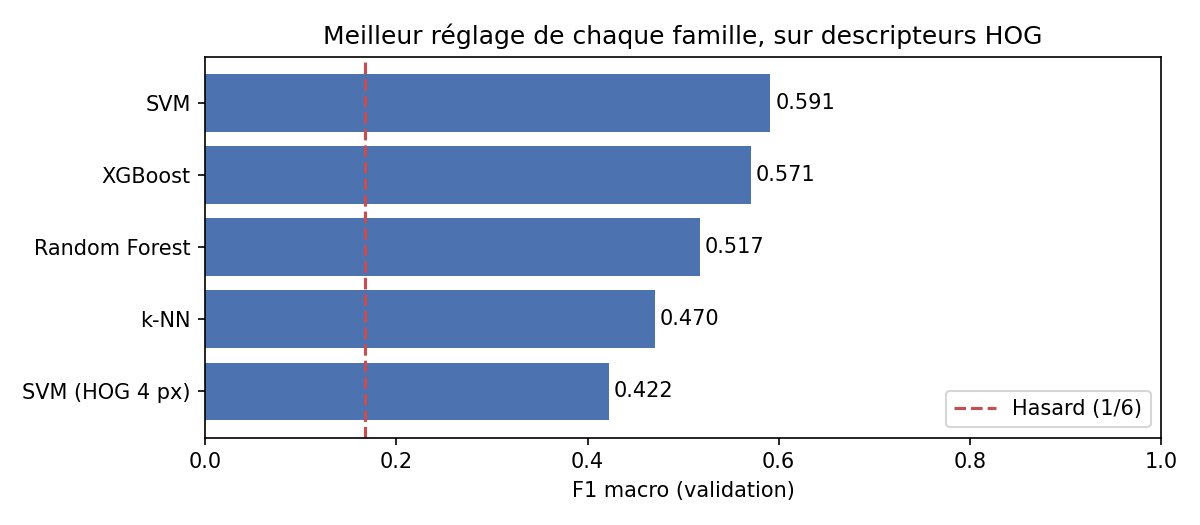
\includegraphics[width=0.72\textwidth]{03_comparaison_familles.png}
  \caption{Comparaison préliminaire sur la validation : meilleur réglage de chaque famille, sur descripteurs HOG. La ligne rouge indique le hasard (1/6).}
  \label{fig:comparaison}
\end{figure}

\textbf{Ce que montrent ces premiers résultats :}

\begin{itemize}
  \item tous les modèles dépassent nettement le hasard ;
  \item le SVM à noyau RBF arrive en tête (0,591), devant XGBoost (0,571), le Random Forest (0,517) et le k-NN (0,470) ;
  \item les confusions principales touchent le camion, souvent pris pour une voiture ou un bus, et le vélo, pris pour une personne ou une moto ;
  \item un premier CNN entraîné de zéro atteint 0,726 en validation. Cette extension reste soumise à l'accord de l'encadrant.
\end{itemize}

\section{Planning de réalisation}
\label{sec:planning}

Le projet dure six semaines, du 4 novembre au 16 décembre 2026. Les dates des séances et du gel du modèle sont fixes ; les durées des travaux restent des estimations. Si une étape prend du retard, ce sont les étapes suivantes qui se décalent, jamais les séances.

\begin{figure}[H]
  \centering
  % Calendrier du 4 novembre au 16 décembre 2026.
% Les dates s'écrivent en nombre de jours depuis le 4 novembre :
% 11 nov. = 7, 13 nov. = 9, 14 nov. = 10, 18 nov. = 14, 20 nov. = 16, 25 nov. = 21,
% 26 nov. = 22, 2 déc. = 28, 9 déc. = 35, 11 déc. = 37, 16 déc. = 42.
\begin{tikzpicture}[x=0.205cm, y=-0.62cm]
  \def\depart{21}     % décalage de l'axe du temps par rapport aux noms (en jours d'échelle)

  % Barre : \tache{ligne}{début}{fin}{nom}{dates}
  \newcommand{\tache}[5]{
    \node[anchor=west, font=\small] at (0,#1) {#4};
    \fill[black!18, draw=black!60, rounded corners=2pt] (\depart+#2,#1-0.22) rectangle (\depart+#3,#1+0.22);
    \node[anchor=west, font=\scriptsize, text=black!70, fill=white, inner sep=1.5pt] at (\depart+#3+0.5,#1) {#5};
  }
  % Jalon : \jalon{ligne}{date}{nom}{dates}{couleur}
  \newcommand{\jalon}[5]{
    \node[anchor=west, font=\small] at (0,#1) {#3};
    \fill[#5] (\depart+#2,#1-0.26) -- ++(0.9,0.26) -- ++(-0.9,0.26) -- ++(-0.9,-0.26) -- cycle;
    \node[anchor=west, font=\scriptsize, text=black!70, fill=white, inner sep=1.5pt] at (\depart+#2+1.2,#1) {#4};
  }

  % Axe du temps, par semaine
  \foreach \jour/\texte in {0/4 nov., 7/11 nov., 14/18 nov., 21/25 nov., 28/2 déc., 35/9 déc., 42/16 déc.} {
    \draw[black!15] (\depart+\jour,0.3) -- (\depart+\jour,10.5);
    \node[font=\scriptsize, text=black!70] at (\depart+\jour,-0.05) {\texte};
  }
  \draw[black!60] (\depart,0.3) -- (\depart+42,0.3);

  \jalon{1}{0}{Go/noGo (séance 1)}{4 nov.}{black!65}
  \tache{2}{0}{14}{Données et recadrages}{4 au 18 nov.}
  \tache{3}{7}{21}{Modèles classiques}{11 au 25 nov.}
  \jalon{4}{9}{Démo du simulateur}{13 nov.}{black!65}
  \tache{5}{10}{16}{Référence, si accord}{14 au 20 nov.}
  \tache{6}{14}{35}{CNN de zéro}{18 nov. au 9 déc.}
  \jalon{7}{21}{Mi-parcours (séance 2)}{25 nov.}{black!65}
  \tache{8}{22}{37}{Évaluation, branchement}{26 nov. au 11 déc.}
  \jalon{9}{35}{\textbf{Modèle figé}}{\textbf{9 déc.}}{accent}
  \jalon{10}{42}{Soutenance}{16 déc.}{black!65}
\end{tikzpicture}

  \caption{Calendrier prévisionnel : le modèle est figé le 9 décembre, une semaine avant la soutenance.}
  \label{fig:planning}
\end{figure}

La figure~\ref{fig:efforts} donne la répartition des efforts que nous visons. Le Machine Learning et les données en prennent la plus grande part, car ils forment le cœur du sujet.

\begin{figure}[H]
  \centering
  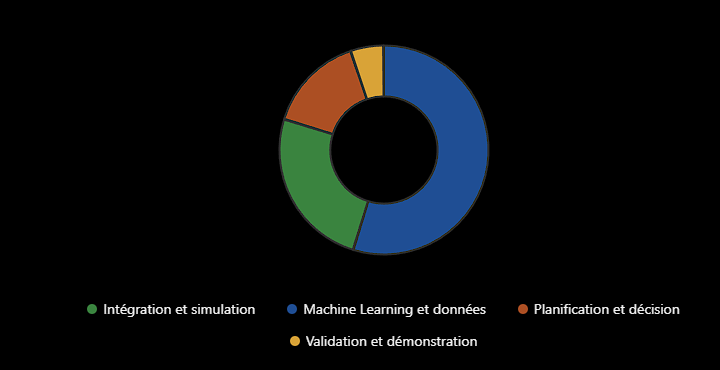
\includegraphics[width=0.6\textwidth]{repartition_indicative_des_efforts.png}
  \caption{Répartition indicative des efforts : c'est une proposition de répartition du travail, pas une mesure du temps déjà passé.}
  \label{fig:efforts}
\end{figure}

\section{Critères de décision Go/noGo}
\label{sec:criteres-go}

\begin{center}
\small
\begin{tabularx}{\textwidth}{>{\raggedright\arraybackslash}p{4.6cm}Y>{\raggedright\arraybackslash}p{1.9cm}}
  \toprule
  \textbf{Critère} & \textbf{Constat} & \textbf{Statut} \\
  \midrule
  Un dataset exploitable existe & COCO couvre les 6 classes ; données préparées & Rempli \\
  Une méthodologie réaliste existe & Protocole fixé, test réservé, métriques définies & Rempli \\
  La classification fonctionne & Tous les modèles dépassent nettement le hasard & Rempli \\
  L'usage des prédictions est défini & Règles de décision et association prédiction--objet décrites & Rempli \\
  L'architecture est cohérente & Modules, échanges et diagrammes définis & Rempli \\
  Les moyens suffisent & Outils gratuits, entraînement possible sans GPU & Rempli \\
  Les choix sont validés par l'encadrant & Trois points restent à confirmer & À valider \\
  \bottomrule
\end{tabularx}
\end{center}

\textbf{Décision demandée : Go.} Pour avancer dans de bonnes conditions, nous avons besoin de l'avis de notre encadrant sur trois points :

\begin{itemize}[label=$\square$]
  \item \textbf{Jeu de données :} COCO 2017 recadré convient-il, avec CIFAR comme solution de secours ?
  \item \textbf{Périmètre :} acceptez-vous XGBoost, le CNN entraîné de zéro et le simulateur comme ajouts au sujet, l'évaluation restant centrée sur SVM, Random Forest et k-NN ?
  \item \textbf{Modèle de référence :} pouvons-nous utiliser un ResNet-18 préentraîné uniquement comme point de comparaison, bien séparé de notre modèle ? Sans accord, nous le retirons, et le reste du plan ne change pas.
\end{itemize}

\chapter*{Conclusion générale}
\addcontentsline{toc}{chapter}{CONCLUSION GÉNÉRALE}

Le projet \textbf{AutoMaze AI} s'inscrit dans une démarche de conception et de développement d'un système de \textbf{classification d'objets routiers par Machine Learning}, destiné à guider les décisions d'un véhicule autonome virtuel. À travers les différentes étapes déjà amorcées, ce travail a permis de poser des bases solides, en définissant clairement les objectifs et le périmètre du projet, en étudiant et en préparant les données, et en concevant une architecture cohérente.

Les choix effectués reposent sur le jeu de données \textbf{COCO 2017}, sur des recadrages carrés de 64~×~64~px et sur un découpage par photo qui évite toute fuite de données. Les trois classifieurs du sujet, \textbf{SVM}, \textbf{Random Forest} et \textbf{k-NN}, seront comparés sur des descripteurs HOG à l'aide du F1 macro. Les prédictions du modèle seront ensuite exploitées par un véhicule virtuel circulant dans les rues de Casablanca, la position des objets étant fournie par le simulateur et leur nature uniquement par le modèle.

Le bilan de faisabilité est encourageant. Les données sont disponibles et préparées, les premiers classifieurs dépassent nettement le hasard, et les moyens nécessaires sont entièrement gratuits. Le projet nous semble donc réalisable dans les délais, sous réserve de l'accord de notre encadrante sur les trois points présentés à la section~\ref{sec:criteres-go}.

Pour la suite, le travail portera sur le réglage des modèles sur la validation, puis sur l'évaluation du modèle final sur le jeu de test et sur de nouvelles images. Si le temps le permet, une attention particulière sera également accordée à l'amélioration des règles de décision, en tenant compte de la distance et de la position des objets, ainsi qu'à l'étude de l'apport d'un CNN entraîné de zéro.

En somme, ce dossier représente une \textbf{phase essentielle de préparation et de structuration} avant la réalisation complète du projet. Il constitue un socle solide pour la mise en œuvre d'un classifieur fiable et pour la démonstration de son utilité dans un contexte de conduite autonome.

\begin{thebibliography}{99}
\addcontentsline{toc}{chapter}{Bibliographie}

\bibitem{coco} T.-Y. Lin, M. Maire, S. Belongie et al., \emph{Microsoft COCO: Common Objects in Context}, European Conference on Computer Vision (ECCV), 2014. \url{https://cocodataset.org}

\bibitem{hog} N. Dalal et B. Triggs, \emph{Histograms of Oriented Gradients for Human Detection}, IEEE Conference on Computer Vision and Pattern Recognition (CVPR), 2005.

\bibitem{svm} C. Cortes et V. Vapnik, \emph{Support-Vector Networks}, Machine Learning, vol.~20, 1995.

\bibitem{rf} L. Breiman, \emph{Random Forests}, Machine Learning, vol.~45, 2001.

\bibitem{knn} T. Cover et P. Hart, \emph{Nearest Neighbor Pattern Classification}, IEEE Transactions on Information Theory, vol.~13, 1967.

\bibitem{xgboost} T. Chen et C. Guestrin, \emph{XGBoost: A Scalable Tree Boosting System}, ACM SIGKDD, 2016.

\bibitem{rcnn} R. Girshick, J. Donahue, T. Darrell et J. Malik, \emph{Rich Feature Hierarchies for Accurate Object Detection and Semantic Segmentation}, CVPR, 2014.

\bibitem{dijkstra} E.~W. Dijkstra, \emph{A Note on Two Problems in Connexion with Graphs}, Numerische Mathematik, vol.~1, 1959.

\bibitem{osm} Contributeurs OpenStreetMap, données sous licence ODbL. \url{https://www.openstreetmap.org}

\bibitem{sklearn} F. Pedregosa et al., \emph{Scikit-learn: Machine Learning in Python}, Journal of Machine Learning Research, vol.~12, 2011.

\bibitem{pytorch} A. Paszke et al., \emph{PyTorch: An Imperative Style, High-Performance Deep Learning Library}, NeurIPS, 2019.
\end{thebibliography}

\appendix

\chapter{Sources des illustrations}
\label{annexe:sources}

Les figures produites par nos notebooks et notre simulateur sont les nôtres. Les autres illustrations viennent de sources externes et servent seulement à illustrer le propos.

\begin{center}
\small
\begin{tabularx}{\textwidth}{>{\raggedright\arraybackslash}p{5.6cm}Y}
  \toprule
  \textbf{Illustration} & \textbf{Source} \\
  \midrule
  Scénarios 1 à 4 & \acompleter{Source et licence à indiquer} \\
  Environnements virtuels (figure~\ref{fig:inspiration}) & \acompleter{Source et licence à indiquer} \\
  Détection par R-CNN (figure~\ref{fig:detection}) & \acompleter{Source et licence à indiquer} \\
  Modèles 3D des classes & Captures de sites de modèles 3D, dont fab.com (moto) et turbosquid.com (voiture) ; \acompleter{auteurs à indiquer} \\
  Flux de développement, répartition des efforts & Schémas réalisés pour le projet \\
  Statistiques, recadrages et comparaison des modèles & Nos notebooks, à partir de COCO 2017 \\
  Capture du simulateur & Notre simulateur ; carte © contributeurs OpenStreetMap (ODbL) \\
  \bottomrule
\end{tabularx}
\end{center}

\chapter{Usage de l'intelligence artificielle}

Le simulateur et la structure des notebooks ont été préparés avec l'aide de Claude Code, et la rédaction de ce dossier a aussi été assistée par cet outil. Les résultats préliminaires de la section~\ref{sec:preuves} et les chiffres du chapitre~\ref{chap:donnees} viennent de notebooks complétés et exécutés par Claude Code sur la branche \texttt{correction} du dépôt, à la demande de l'équipe. Nous les présentons comme des preuves de faisabilité. Leur place dans le travail noté reste à définir avec notre encadrant.


\end{document}
